\graphicspath{{img/ch3/}}
\cleardoublepage
\chapter{Model Order Reduction of Phased Array Antennas} \label{chap:MOR}

\par Even with the immense computing power nowadays available, the electromagnetic modeling of electrically large structures, due to their high computational resources demand, still remains a challenge. Techniques such as the \itt{domain decomposition} \cite{GuarnieriSelleriFEDD, SelleriEdlingerDDMOR} may be used in order to split a large computational domain into smaller ones, reducing in this way the memory requirements and the overall computational time. The finite elements analysis of arbitrarily shaped radiating structures is usually achieved by the decoupling of the finite elements formulation, that is a system of differential equations stated in a weak form to obtain a linear system of equations, from the boundary integrals required to compute the radiated far fields from equivalent surface currents. Thus the finite elements domain is limited to the near fields region, truncating the finite elements domain such that the memory requirements become acceptable. Then the fields computed on a surface bounding the radiating elements allow the computation of the radiated fields with the near fields to far fields transformations stated by the integrals presented in chapter \ref{chap:N2F}.

\par The Petrov-Galerkin projections \cite{ThomeeGFEMP} on the finite elements differential equations leads to a linear system of equations in which the unknowns are the coefficients for the chosen basis expansion. This linear system can be thought as the input linear system of equations of a radiating model, and the spanning coefficients of the basis as a \itt{state vector}. Then, an output system of equations, based on the N2F operator introduced in chapter \ref{chap:LRA},  modified in order to act on the state vector, completes the modeling of an analyzed radiating structure.

\par The full system obtained in such a way is composed by very large but sparse matrices, typically with hundred thousands and even hundred millions of unknowns. The application of projection based model order reduction techniques, leading to full matrices but of several orders of magnitude lower, allows fast on-line stage computations. Furthermore, the approximations made in the far-fields operators through the DFT-truncation allow to minimize the size of the system output matrix, especially for very large planar arrays.

\par In a first part of this chapter, the general FEM formulation for the input system matrices will be viewed, together with the construction of the output system matrices, in order to build the full radiation model. Then, the choice of the approximation spaces for the near fields will be discussed for the model order reduction, keeping particular attention on the error introduced. Finally, the effectiveness of a model order reduction applied to two different radiating structures will be shown, comparing the results to the full-model computations.

%%%%%%%%%%%%%%%%%%%%%%%%%%%%%%%%%%%%%%%%%%%%%%%%%%%%%%%%%%%%%%%%%%%%%%%%%%%%%%%%
\section{The FEM vector Helmholtz formulation}

\par The most commonly employed formulation of the full-wave finite elements for solving the Maxwell's equations in a bounded domain is the vector Helmholtz equation for the electric field, recast in a weak form (\itt{weighted residuals}) to achieve a linear equations system. The weak form is supplied by the testing of \eqref{eq:waveE} with opportune basis, the \itt{curl-conforming vector finite elements}\footnote{Initially introduced by N\'{e}d\'{e}lec, then developed by the research community into the so-called \itt{hierarchical finite element basis} for vector fields.}. Consider the domain $\mrm{\Omega} \subset \mathbb{R}^3$ to be bounded by $\mrm{\partial \Omega = \Gamma = \Gamma_E \cup \Gamma_{H} \cup \Gamma_{WG} \cup \Gamma_R}$ as depicted in figure \ref{fig:FEMproblem}.
\begin{figure}[hbpt!]
\centering
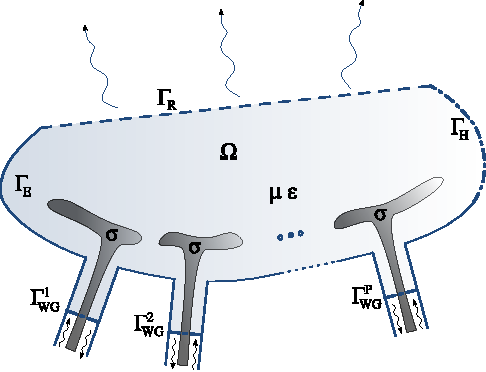
\includegraphics[width=12cm]{FEMproblem} 
\caption{FEM domain of the radiation problem.}
\label{fig:FEMproblem}
\end{figure}
$\mrm{\Gamma}_E$ corresponds to {Dirichlet conditions} boundaries, $\mrm{\Gamma}_H$ to {Neumann conditions} boundaries, $\mrm{\Gamma}_{WG}$ to waveguides truncation boundaries, and $\mrm{\Gamma}_R$ is the radiation boundary. Consider now the discretized domain $\mrm{\Omega}_h = \bigcup_{n=1}^{N} \mrm{\Omega}_n \subset \mrm{\Omega}$, where the subdomains $\mrm{\Omega}_n$ (the  tetrahedra for example) are such that $\mrm{\Omega}_n \cap \mrm{\Omega}_m = \{ 0 \}$ for $n \neq m$. $\mrm{\Omega}_h$ is parameterized in by the maximum diameter $h$ of the subdomains $\mrm{\Omega}_n$, and we shall assume that as $h \to 0$, $\mrm{\Omega}_h \to \mrm{\Omega}$. With $\hat{\mbfit{n}}$ pointing outwardly from $\mrm{\Omega}$, consider the \itt{Sobolev} space \cite{MonkFEME} $\mcal{W} = \mcal{W}(\mrm{\Omega}_h) \subset \mcal{H}(\mrm{curl}; \mrm{\Omega})$ of the \itt{trial} functions $\mbfit{w}$, defined by the direct sum of two closed subspaces as follows
\begin{eqnarray}
\mcal{W} &= & \mcal{W}_D \oplus \mcal{W}_E, \nonumber \\
\mcal{W}_D &:= & \{ \mbfit{w} \in \mcal{W}| \hat{\mbfit{n}} \times \mbfit{w} = 0 \ \mrm{on} \ \mrm{\Gamma}_E \} \subset \mcal{H}(\mrm{curl;\mrm{\Omega}}), \nonumber \\
\mcal{W}_E &:= & \{ \mbfit{w} \in \mcal{W}| \hat{\mbfit{n}} \times \mbfit{w} \neq 0 \ \mrm{on} \ \mrm{\Gamma}_E \} \subset \mcal{H}(\mrm{curl;\mrm{\Omega}, \mrm{\Gamma}_E}).
\end{eqnarray} $\mcal{W}_D$ is in fact the subspace of the imposed Dirichlet conditions. The total electric field is given by the approximating finite summations
\begin{eqnarray}
\label{eq:fieldExp}
\mbfit{E} & = & \hat{\mbfit{E}} + \mbfit{E}_D, \nonumber \\
\hat{\mbfit{E}} &:= & \sum_i x_i \mbfit{w}_i, \qquad \mbfit{w}_i \in \mcal{W}_E, \nonumber \\
\mbfit{E}_D&:= & \sum_j x_j \mbfit{w}_j, \qquad \mbfit{w}_j \in \mcal{W}_D.
\end{eqnarray} With Galerkin projections (the test functions are the same as the trial functions), it is possible to construct an algebraic linear system with as unknowns only the coefficients $x_i$. In effect, $x_j$ are not problem unknowns as they are given by the boundary conditions.

\par Now, as $\mrm{\Omega}$ does not contain any impressed current sources, only induced currents persist and \eqref{eq:waveE} can be rewritten as \cite{FarleMORFE}
\begin{eqnarray}
\nabla \times \frac{1}{\mu_r} \nabla \times \mbfit{E} + jk_0\zeta_0\sigma \mbfit{E}  - k_0^2\epsilon_r \mbfit{E}  =  0,
\end{eqnarray}  with $k_0 = \omega \sqrt{\epsilon_0 \mu_0}$ the free space wave number and $\zeta_0$ the free space plane wave impedance. For notation disambiguation, notice that the formulation presented is a frequency-domain one, and the spectrum $\tilde{\mbfit{E}}(\mbfit{r},\omega)$ has to be computed by means of a frequency sweep. Thus, consider $\tilde{\mbfit{E}}(\mbfit{r},\omega) \Big |_{\omega = \omega_n} = \mbfit{E}$ to be the electric field at a given angular frequency $\omega_n$. The boundary conditions can be stated as
\begin{eqnarray}
\hat{\mbfit{n}} \times ( {\mbfit{E}} \times \hat{\mbfit{n}}) & = & \bar{\mbfit{E}}_t, \qquad \mrm{on} \ \mrm{\Gamma}_E, \nonumber \\
\hat{\mbfit{n}} \times ( {\mbfit{H}} \times \hat{\mbfit{n}}) & = & \bar{\mbfit{H}}_t, \qquad \mrm{on} \ \mrm{\Gamma}_{H}, \nonumber \\
\hat{\mbfit{n}} \times ( {\mbfit{E}} \times \hat{\mbfit{n}}) & = & Z_s {\mbfit{H}} \times \hat{\mbfit{n}}, \qquad \mrm{on} \ \mrm{\Gamma}_R, \nonumber \\
\hat{\mbfit{n}} \times ( {\mbfit{H}} \times \hat{\mbfit{n}}) & = & \sum_{k} \left ( a_k^i - a_k^r \right ) \mbfit{H}_t^k, \qquad \mrm{on} \ \mrm{\Gamma}_{WG},
\end{eqnarray} $\bar{\mbfit{E}}_t$ and $\bar{\mbfit{H}}_t$ known values, $Z_s$  the wave impedance at the radiation boundary, and $a_k^i, a_k^r$ the $k^\mrm{th}$ complex modal incident and reflected amplitudes . We proceed with the Galerkin projections, obtaining \cite{FarleMORFE}
\begin{eqnarray}
\label{eq:FEMform}
\int_\mrm{\Omega} \nabla \times \mbfit{w}_i \cdot \frac{1}{\mu_r} \nabla \times \mbfit{E} \ d\mrm{\Omega} + j k_0 \zeta_0 \int_\mrm{\Omega} \mbfit{w}_i \cdot \sigma \mbfit{E} d\mrm{\Omega} \ + \nonumber \\
 j k_0 \zeta_0 \int_{\mrm{\Gamma}_R} \hat{\mbfit{n}} \times \mbfit{w}_i \cdot \frac{1}{Z_s} \hat{\mbfit{n}} \times \mbfit{E} d\mrm{\Gamma} - k_0^2 \int_\mrm{\Omega} \mbfit{w}_i \cdot \epsilon_r \mbfit{E} d\mrm{\Omega} \nonumber \\
\hspace{-10cm} = j k_0 \zeta_0 \int_{\mrm{\Gamma}_{WG}} \mbfit{w}_i \cdot \hat{\mbfit{n}} \times \mbfit{H}_t d\mrm{\Gamma}, \qquad \forall \mbfit{w}_i \in \mcal{W}_E.
\end{eqnarray} On $\mrm{\Gamma}_{WG}$, if we consider the wave ports to be fed only by the dominant mode (lowest cutoff frequency), the following relation holds for the $k^\mrm{th}$ port \cite{PelosiCoccioliSelleriQFEEF, ZhuCangellarisMFEMEFM}
\begin{eqnarray}
\hat{\mbfit{n}} \times \mbfit{H}_t^k & = & \frac{1}{Z_k} \hat{\mbfit{n}} \times \hat{\mbfit{n}} \times \mbfit{E}_t^k - \frac{2}{Z_k} \hat{\mbfit{n}} \times \hat{\mbfit{n}} \times \mbfit{E}_t^{k \ \mrm{inc}}, \qquad \mrm{on} \ \mrm{\Gamma}_{WG}^k,
\end{eqnarray} where $\mbfit{E}_t^{k \ \mrm{inc}}$ is the incident electric field and ${Z_k}$ the modal impedance. Assuming the waveguides segments on which the wave ports are applied to be long enough such that the higher order modes are evanescent and once they encounter the electromagnetic structure's discontinuities (e.g. the junction to the antenna) their power contribution is several order of magnitude lower than the one of the dominant mode, this so-called \itt{transfinite elements method} \cite{ZhuCangellarisMFEMEFM} allows to feed a generic structure though waveguides and \eqref{eq:FEMform} becomes 
\begin{eqnarray}
\label{eq:FEMformTFE}
& & \hspace{-1.5cm} \int_\mrm{\Omega} \nabla \times \mbfit{w}_i \cdot \frac{1}{\mu_r} \nabla \times \mbfit{E} \ d\mrm{\Omega} + j k_0 \zeta_0 \int_\mrm{\Omega} \mbfit{w}_i \cdot \sigma \mbfit{E} d\mrm{\Omega} \ - \nonumber \\
& &\hspace{-1cm} k_0^2 \int_\mrm{\Omega} \mbfit{w}_i \cdot \epsilon_r \mbfit{E} d\mrm{\Omega} + j k_0 \zeta_0 \int_{\mrm{\Gamma}_R} \hat{\mbfit{n}} \times \mbfit{w}_i \cdot \frac{1}{Z_s} \hat{\mbfit{n}} \times \mbfit{E} d\mrm{\Gamma} + \nonumber \\
& & \hspace{-.5cm}\sum_{m=1}^M \frac{j k_0 \zeta_0}{Z_m} \int_{\mrm{\Gamma}_{WG}^m} \hat{\mbfit{n}} \times \mbfit{w}_i \cdot \hat{\mbfit{n}} \times \mbfit{E}_t d\mrm{\Gamma} \nonumber \\
& & \hspace{0cm} = \frac{j 2 k_0 \zeta_0}{Z_k} \int_{\mrm{\Gamma}_{WG}^k} \hat{\mbfit{n}} \times \mbfit{w}_i \cdot \hat{\mbfit{n}} \times \mbfit{E}_t^{k \ \mrm{inc}}  d\mrm{\Gamma}, \qquad \forall \mbfit{w}_i \in \mcal{W}_E
\end{eqnarray} where $M$ is the total number of ports and $1 \leq k \leq M$. The present formulation, for the summation all over the ports entering into the computational domain, couples one port to the others, hence models the mutual couplings between the radiating elements.
The condition on $\mrm{\Gamma}_R$ is an impedance condition, the so-called \itt{absorbing boundary condition} (ABC), which ideally annihilates the locally plane wave reflection on the boundary. Actually, the reflection coefficient is strongly dependent on the incidence angle of the plane wave, being null for perpendicular one. In order to keep sufficient validity in the computation of the fields in opened structures, the ABCs must be placed sufficiently far away from the radiating elements or scatterers such that incidence becomes less oblique. For example, in the commercial CAD HFSS\footnote{Ansoft $\mrm{HFSS}^{\textrm{\texttrademark}}$ (acquired by Ansys Inc.). Further informations available at \url{http://www.ansys.com/products/electromagnetics/}.}, the recommendations are to place the radiation boundaries at least at $\nicefrac{\lambda_\mrm{min}}{2}$ away from the radiating sources, where $\lambda_\mrm{min}$ is associated to the highest frequency set in a frequency sweep.

\par Equation \eqref{eq:FEMformTFE} leads, with the field expansion of \eqref{eq:fieldExp} and setting the solving frequency ($k_0 = \omega\sqrt{\epsilon_0 \mu_0}$), to $M$ linear systems associated to each port of the form \cite{JinFEME,PelosiCoccioliSelleriQFEEF} 
\begin{eqnarray}
\label{eq:inSystem}
\mat{A} \ \vect{x}  & = & \vect{b},
\end{eqnarray} where $\mat{A} \in \mathbb{C}^{N \times N}$ is a symmetric matrix, $\vect{x}, \vect{b} \in \mathbb{C}^{N}$ and $N$ the number of unknowns or \itt{degrees of freedom} (DoFs).
\par The system of \eqref{eq:inSystem} is such that, in the case we are analyzing an electrically large structure, $N$ is in the order of hundred thousands to several millions. This is due to the fact that the size of the elements $h$ has to be very low respectively to the wavelength in order to reduce the fields \itt{jumps} from one element to a neighboring one. Typical values are comprised between $\nicefrac{\lambda}{3}$ and $\nicefrac{\lambda}{10}$ in order to keep sufficient accuracy while not exceeding in the computational resources demand. Also, when using higher order polynomials to approximate the fields, as the number of basis functions increase, the number of unknowns or DoFs increase. Where the fields are known to vary rapidly, e.g. next to fields singularities of a conducting plate, the size of the elements must be lowered to achieve better accuracy. All these factors have to be taken into account for an effective design, and the final system dimension depends on them.
%%%%%%%%%%%%%%%%%%%%%%%%%%%%%%%%%%%%%%%%%%%%%%%%%%%%%%%%%%%%%%%%%%%%%%
\section{Projection-based model order reduction}

\begin{mydef}
Consider the single input, single output (SISO) polynomially parameterized full system
\begin{eqnarray}
\label{eq:fullSISO}
\mat{A} \ \vect{x} (p)  & = & \left ( \sum_{i=1}^{M} \Theta_i(p) \ \vect{b}_i \right ) u(p),\nonumber \\
y(q) &= & \left ( \sum_{j=1}^{Q} \Omega_j(q) \ \vect{c}^H_j \right ) \ \vect{x} (p),
\end{eqnarray} with $\mat{A} \in \mathbb{C}^{N \times N}$, $\vect{x}, \vect{b}_i, \vect{c}_j \in \mathbb{C}^{N}$, $\vect{b}_i$ being the $i^\mrm{th}$ system input vector, $\vect{c}_j$ the $j^\mrm{th}$ output vector, $\Theta_i(p)$ the $i^\mrm{th}$ term of the polynomial parameterization in $p$ of the input system equation and $\Omega_j(p)$ the $j^\mrm{th}$ term of the polynomial parameterization in $q$ of the output system equation. The projection-based reduced order model (ROM) is given by \cite{FarleMORFE}
\begin{eqnarray}
\label{eq:ROMSISO}
\tilde{\mat{A}} \ \tilde{\vect{x}} (p) & = & \left ( \sum_{i=1}^{M} \Theta_i(p) \ \tilde{\vect{b}}_i \right )  u(p),\nonumber \\
y(q) &= & \left ( \sum_{j=1}^{Q} \Omega_j(q) \ \tilde{\vect{c}}^H_j \right ) \ \tilde{\vect{x}} (p),
\end{eqnarray} with
\begin{eqnarray}
\label{eq:ProjectedSISO}
\tilde{\mat{A}} & := & \mat{W}^H \mat{A} \mat{V} \nonumber \\
\tilde{\vect{b}}_i & := & \mat{W}^H \vect{b}_i,\nonumber \\
\tilde{\vect{c}}_j & := & \mat{V}^H \vect{c}_j,
\end{eqnarray} and $\mat{W}, \mat{V} \in \mathbb{C}^{N \times n}, \ n \ll N$.
\end{mydef}
The full unknowns vector is approximated by $\vect{x} \approx \mat{V} \tilde{\vect{x}}$, that is $\vect{x}$ is spanned by the column space of $\mat{V}$ (trial vectors) through the coefficients $\tilde{\vect{x}}$ computed from the solution of the ROM input system. Thus, $\mat{V}$ constitute a set of global basis vectors for the full FEM system. $\mat{W}^H$ applied to the column vectors of a matrix or to a vector is a testing operation with the space spanned by the columns of $\mat{W}$ (see chapter \ref{chap:LRA}).

%\par The SISO system of \eqref{eq:fullSISO} is actually the model of a single phased array, or a group of antennas that constitute a phased array. In order to handle more groups of phased arrays to redefine the full model into the following multiple inputs, multiple outputs (MIMO) form
%\begin{eqnarray}
%\label{eq:fullMIMO}
%\mat{A}_i \ \vect{x} (p)  & = & \left ( \sum_{i=1}^{M} \Theta_i(p) \ \mat{B}_i \right ) \vect{u}(p), \nonumber \\
%\vect{y}(p) &= & \left ( \sum_{i=1}^{M} \Theta_i(p) \ \mat{C}^H_i \right ) \ \vect{x} (p),
%\end{eqnarray} with $\vect{x} \in \mathbb{C}^N, \vect{u} \in \mathbb{C}^g, \vect{y} \in \mathbb{C}^h$, $\mat{A}_i \in \mathbb{C}^{N \times N}$, $\mat{B}_i \in \mathbb{C}^{N \times g}, \mat{C}_i \in \mathbb{C}^{h \times N}$, and $\Theta_i(p)$ is the $i^\mrm{th}$ term of the polynomial parameterization in $p$. Thus, the ROM of the present model is given by
%\begin{eqnarray}
%\label{eq:ROMMIMO}
%\left ( \sum_{i=1}^{M} \Theta_i(p) \ \tilde{\mat{A}}_i \right ) \ \tilde{\vect{x}} (p) & = & \left ( \sum_{i=1}^{M} \Theta_i(p) \ \tilde{\mat{B}}_i \right ) \vect{u} (p),\nonumber \\
%\vect{y} (p) &= & \left ( \sum_{i=1}^{M} \Theta_i(p) \ \tilde{\mat{C}}^H_i \right ) \ \tilde{\vect{x}} (p),
%\end{eqnarray} with
%\begin{eqnarray}
%\label{eq:ProjectedMIMO}

%\tilde{\mat{A}}_i & := & \mat{W}^H \mat{A}_i, \mat{V} \nonumber \\
%\tilde{\mat{B}}_i & := & \mat{W}^H \mat{B}_i,\nonumber \\
%\tilde{\mat{C}}_i & := & \mat{V}^H \mat{C}_i,
%\end{eqnarray} and $\mat{W}, \mat{V} \in \mathbb{C}^{N \times n}, \ n \ll N$.

%%%%%%%%%%%%%%%%%%%%%%%%%%%%%%%%%%%%%%%%%%%%%%%%%%%%%%%%%%%%%%%%%%
\section{Scan and look angles parameterized radiation model}

\par The full system \eqref{eq:fullSISO} represents our electromagnetic model of a phased array. Each column vector $\mat{b}_i$ represent a different right-hand side of the system, considering one by one each of the $g$ excitation ports. In effect, with \eqref{eq:FEMformTFE} the right-hand side is build for each k with $1 \leq k \leq M=g$, one by one while looking at the fields, that is the unknowns to find, produced by the excitations taken singularly. The superposition of the solutions, as the system is invariant ($\mat{A}$ remains the same all along this process), gives the fields produced by the ports excited contemporaneously. This is obvious if we think of the linearity property of the system. Now, as we are seeking for a beam steering operation, and we know that it is achieved by relative phase shifts between the excitations given by \eqref{eq:Excitations}, the polynomial terms are given by $\Theta (\theta_x,\theta_y) = \left \{  a_i \ \mrm{e}^{-jk ( x_i \sin(\theta_{x}) + y_i \sin(\theta_{y}))}, 1 \leq i \leq g \right \}$ where $a_i \in \mathbb{C}$ is complex coefficient that can be devoted to pattern shaping \cite{SelleriETA, MilliganMAD} or left to 1 if we desire only the beam steering. We can rewrite the right-hand side of the input equation of \eqref{eq:fullSISO} as the sum of coefficient-vector products
\begin{eqnarray}
\label{eq:scanAngle}
\mat{A} \ \vect{x}  & = & a_1 \ \mrm{e}^{-jk ( x_1 \sin(\theta_{x}) + y_1 \sin(\theta_{y}))} \ \vect{b}_1 + \ldots + a_g \ \mrm{e}^{-jk ( x_g \sin(\theta_{x}) + y_g \sin(\theta_{y}))} \ \vect{b}_g,
\end{eqnarray} emphasizing the parameterization of the system by the scan angle $(\theta_{x}, \theta_{y})$. We have reduced this way the inputs variability to only two values, that is the scan angles in both $x$ and $y$ directions. 

\par The output equation now has to be formulated in such a way that, from the solutions computed by the input equations, we derive the fields in several sampling points surrounding the array, then, applying the N2F operator we obtain the sought spherical components of the far fields detectors. Thus, we build a \itt{solutions-to-fields} operator $\mathcal{F}(x)$ which can be viewed as a large (as large as the unknowns) but sparse matrix that opportunely selects the solutions related to the elements in which the fields have to be sampled, then using them in the expansion \eqref{eq:fieldExp}, recovers the vector fields, electric and magnetic, in each selected point providing for example their Cartesian components. Notice that, for Faraday's law \eqref{eq:ffaraday} and the constitutive relation \eqref{eq:ffsconst2}, the magnetic field is derived from the electric field by a curl operation. Then, from the near fields we can apply our N2F operator $\mathcal{L}(\cdot; \theta)$ (having opportunely included in the operator \eqref{eq:KottlerEN2Fapprox} the $\hat{\mbfit{n}} \times \cdot$ operation on the fields to achieve the tangential components, that is the equivalent currents, and the Cartesian to spherical transformation of note \ref{fn:cart2sph}) to the operator $\mathcal{F}(x)$, that is  $\mathcal{L}(\mathcal{F}(x); \theta)$  to obtain the far fields detectors in the look angle direction $\theta$ for the chosen $\phi$ plane. As we have chosen to supply a DFT-truncation in order to reduce the dimensions of the output operator, the operator $\mathcal{L}(\cdot; \theta)$ is now given by the approximation \eqref{eq:DFTtrunc}, such that the rows are given by the $c = 2 R + 1$ coefficients chosen in the expansion. We can thus write the output matrix as
\begin{eqnarray}
& & \mat{c}_j = \mrm{col}_j \left ( \mat{F}^H \ \tilde{\mat{X}}^H \right ) \ \Omega_j^\dagger (\theta) = \mat{c}'_j \ \Omega_j^\dagger (\theta), \nonumber \\
& & \hspace{-.5cm} \mat{F} \in \mathbb{C}^{l \times N}, \tilde{\mat{X}} \in \mathbb{C}^{1 \times l}, \mat{c}'_j \in \mathbb{C}^{N \times 1}, 1 \leq j \leq Q = c,
\end{eqnarray} with $\Omega (\theta) = \left \{1, \mrm{e}^{j \theta }, \ldots, \mrm{e}^{j R \theta }, \mrm{e}^{- j R \theta}, \ldots,  \mrm{e}^{- j \theta} \right \}$ the polynomial terms of the output system parameterized in the look angle $\theta$. $l$ is the number of vector components for all the sampling points, that is 6 times the number of sampling points. To handle the $\theta$ and $\phi$ polarizations, it is necessary to provide two different DFT coefficients matrices $\mat{X}_\phi$ and $\mat{X}_\theta$, computing separately the far field detectors in each polarization, here considered in the only output $y$. The full system of the radiating model can be stated as
\begin{eqnarray}
\label{eq:fullRadMod}
\mat{A} \ \vect{x}  & = & a_1 \ \mrm{e}^{-jk ( x_1 \sin(\theta_{x}) + y_1 \sin(\theta_{y}))} \ \vect{b}_1 + \ldots + a_g \ \mrm{e}^{-jk ( x_g \sin(\theta_{x}) + y_g \sin(\theta_{y}))} \ \vect{b}_g \nonumber \\
y &= & \left ( {\mat{c}'}_{1}^{H} + \ldots + \mrm{e}^{j R \theta } {\mat{c}'}_{R+1}^{H} \  + \mrm{e}^{-j R \theta } {\mat{c}'}_{R+2}^{H} + \ldots + \mrm{e}^{-j \theta} {\mat{c}'}_{2R+1}^{H} \right )  \vect{x}, \nonumber \\
\vect z &= & \mat F \ \vect{x}.
\end{eqnarray} The power radiated may be computed separately using \eqref{eq:Pr}, considering the near fields ($\vect z$) obtained by $\mat{F} \ \vect{x}$, with $\mat F$ a \itt{solutions-to-near-fields} operator. According to \cite{HuynPateraRBStress}, it is be possible to include the power radiated computation into the output functional $\mathcal{L}(\mathcal{F}(x); \theta)$, combining the power reflected a the ports and the power losses that may occur in dispersive media. Notice that the total power radiated vary during the beam steering operation, the mutual couplings varying as the excitations change, thus has to be computed for each scan angle selected. Finally, the directivity patterns are derived using \eqref{eq:patternForm1} and \eqref{eq:patternForm2}. A model schematic is illustrated in figure \ref{fig:FullRadModel}.
\begin{figure}[hbpt!]
\centering
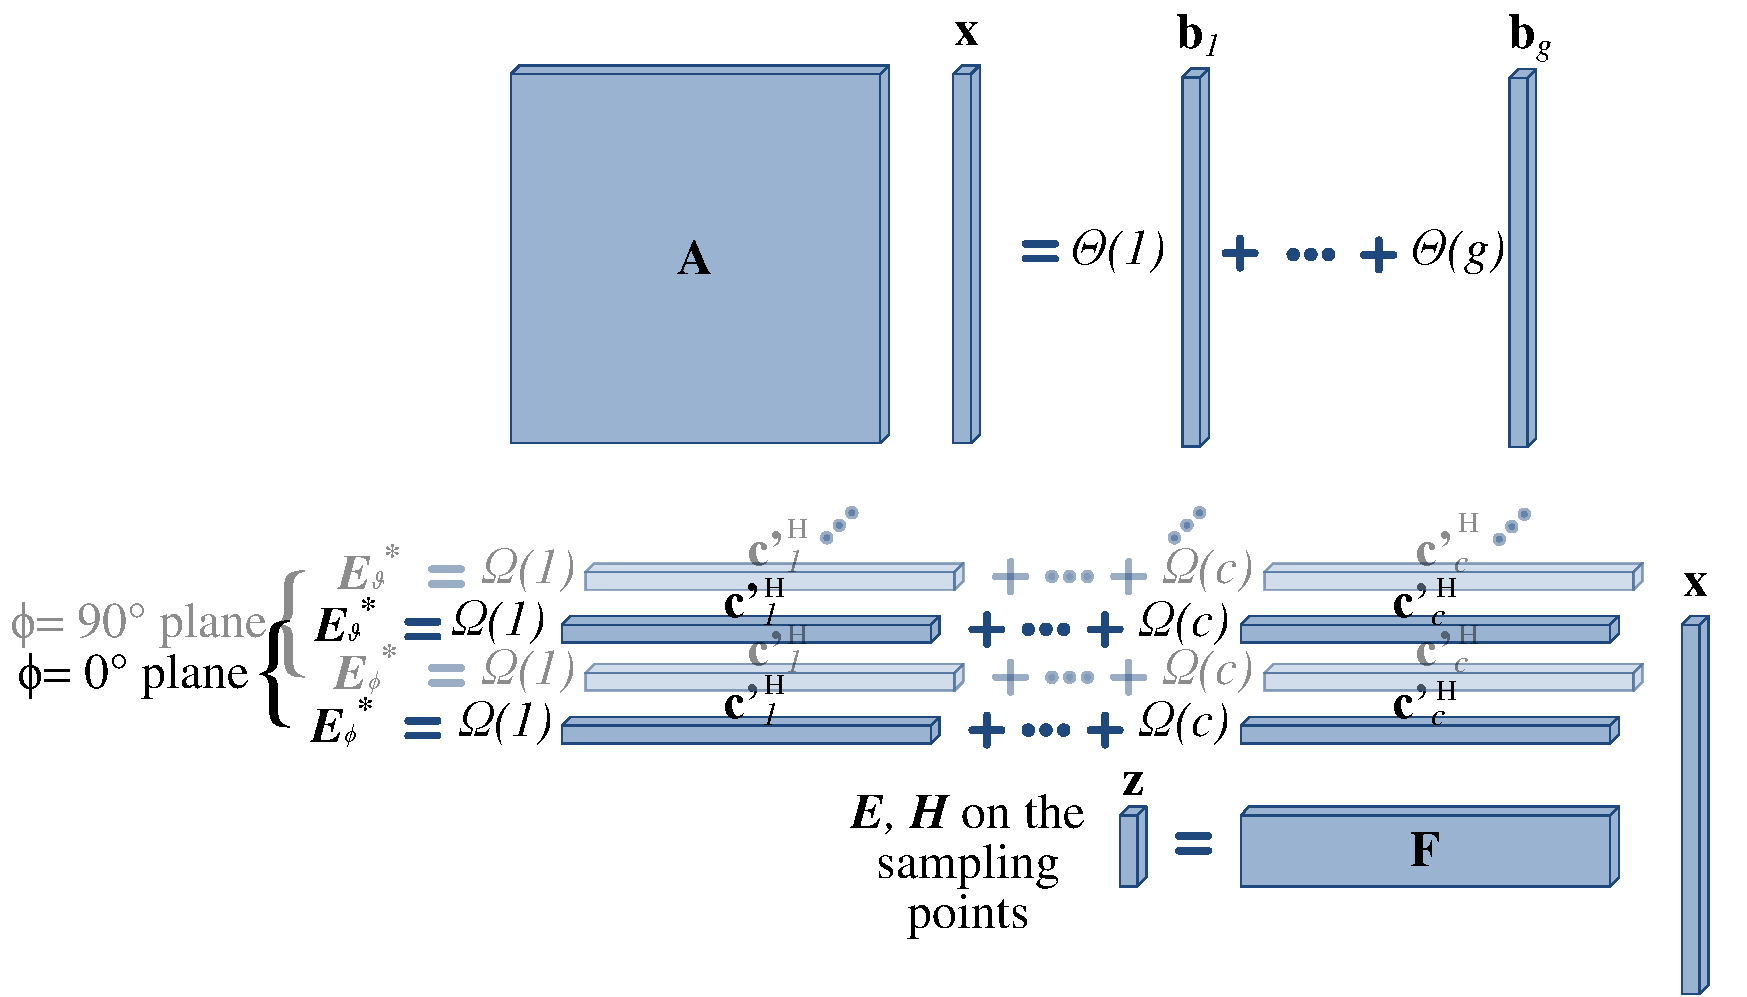
\includegraphics[width=14cm]{FullRadModel} 
\caption{Schematic of the full radiation model.}
\label{fig:FullRadModel}
\end{figure}

\par We proceed applying the model order reduction definition \eqref{eq:ROMSISO} to the SISO-system of \eqref{eq:fullRadMod}:
\begin{eqnarray}
\label{eq:ROMRadMod}
\tilde{\mat{A}} \ \tilde{ \vect{x}}  & = & a_1 \ \mrm{e}^{-jk ( x_1 \sin(\theta_{x}) + y_1 \sin(\theta_{y}))} \ \tilde{ \vect{b}}_1 + \ldots + a_g \ \mrm{e}^{-jk ( x_g \sin(\theta_{x}) + y_g \sin(\theta_{y}))} \ \tilde{\vect{b}}_g \nonumber \\
y &= & \left ({\tilde{\mat{c}}{'}}_{1}^{H} + \ldots + \mrm{e}^{j R \theta }  {\tilde{\mat{c}}{'}}_{R+1}^{H} \  + \mrm{e}^{-j R \theta } { \tilde{\mat{c}}{'}}_{R+2}^{H} + \ldots + \mrm{e}^{-j \theta} {\tilde{\mat{c}}{'}}_{2R+1}^{H} \right ) \tilde{\vect{x}}, \nonumber \\
\vect z &= & \tilde{ \mat F} \ \tilde{\vect{x}}.
\end{eqnarray} where the reduced order matrices of the system are $\tilde{\mat{A}} = \mat{W}^H \ \mat{A} \ \mat{V}, \tilde{\mat{b}}_i = \mat{W}^H \ \mat{b}, \tilde{\mat{c}}{'}_j = \mat{V}^H \ \mat{c}{'}_j$ or analogously, doing the transpose conjugate in both hand-sides, $\tilde{\mat{c}}{'}_j^H = \mat{c}{'}_j^H \ \mat{V}$,  $\tilde{\mat{F}} = \mat{F} \ \mat V$, and $\mat{W}, \mat{V} \in \mathbb{c}^{N \times n}, \ n \ll N$, are respectively trial and test matrices we need to define in order to properly reduce the model.

%%%%%%%%%%%%%%%%%%%%%%%%%%%%%%%%%%%%%%%%%%%%%%%%%%%%%%%%%
\section{Proper choice of the trial and test spaces}

\par The model order reduction is mainly based on the fact that we approximate the solutions as $\vect x = \mat V \tilde{\vect x}$. If $\mat V$ is an orthonormal basis, then $\tilde{\vect x} =  \mat{V}^H \vect x$ and this means to test the solutions vector with an orthonormal basis, i.e. to provide a change of basis, and the testing returns the coefficients $\tilde{\vect x}$ for the expansion in terms of this new basis. Now, to choose $\mat V$, we need to think of what we are testing. The solutions vector is straightly related to the fields by the expansion \eqref{eq:fieldExp}. They are in fact the coefficients of the expansion in terms of orthogonal shape functions that approximates the near fields. Hence, from the results obtained from chapter \ref{chap:LRA}, section \ref{sec:approxNF}, we can express the near fields pictures to span the testing space in terms of solutions obtained for various scan angles. 
%\par Now, as the input system equation is linear, to apply scalar values $u(i), \ 1 \leq i \leq g$ to the right-hand side vectors $\vect{b}_i \subset \mat {B}$ gives the same results as applying the same coefficients to the solutions vectors $\vect{x}_i^{'}$ relative to $\vect{b}_i$ :
%\begin{eqnarray}
%& &\hspace{-.5cm} \mat A \ \vect x = \mat B \ \vect u \ \Rightarrow \ \sum_{i=1}^{g} \mat A \ \vect{x}_i = \sum_{i=1}^{g} \vect{b}_i \ u(i) \ \Rightarrow \ \sum_{i=1}^{g} \vect{x}_i =  \sum_{i=1}^{g} \left ( \mat{A}^{-1} \ \vect{b}_i \right ) \ u(i) = \sum_{i=1}^{g} \vect{x}_i^{'} \ u(i), \nonumber \\
%& &\hspace{3cm} u(i) = u(i; \theta_x, \theta_y).
%\end{eqnarray} We can thus compute in a prior stage the solutions vectors $\vect{x}_i^{'}, \ 1 \leq i \leq g$ corresponding to equal phase for all the excitations, i.e. a broadside radiation configuration. Then, the remaining scan angle selection is done changing the vector $\vect u$ values selecting the appropriate $(\theta_x, \theta_y)$ in \eqref{eq:Excitations}. 

\par We need to collect several linearly independent \itt{solutions pictures} to span the scan angle space. Using the input system of \eqref{eq:fullRadMod}, we compute $\alpha$ solutions $\vect{x}_\alpha$ for a set of $\alpha$ scan angles $(\theta_x, \theta_y)_\alpha$. The dimension of the scan angle space, as it was shown in chapter \ref{chap:LRA}, depends on the array structure: the relative spacing an the number of radiating elements are the principal parameters. To compute the orthonormal vectors $\mat V$, either the SVD (right singular vectors) or the QR factorization (with $\mat Q$ a matrix of orthonormal column vectors) \cite{TrefethenBauNLA} can be used, depending on the number of solutions pictures collected. In effect the complexity of an SVD is in the order of \texttildelow $2 m n^2 + 11 n^3$ while the QR factorization requires \texttildelow $2 m n^2$, where $m$ here corresponds to the DoFs while $n$ is the number of scan angle pictures selected. For large $n$, the QR has a lower cost than the SVD, however with the QR we pay the price that the factorization is not always accurate \cite{TrefethenBauNLA}.

\par The trial space can, in a first attempt, be the same as the testing space, leading to a Galerkin projection. Thus if we chose $\mat W = \mat V$, we may expect a total matching for the scan angles selected and for the remaining scan angles an approximated solution. Thus we can define the trial and test spaces as
\begin{eqnarray}
\mrm{span} \ \left \{ \bigcup_{i=1}^\alpha  \ \vect{x}_i(\theta_x, \theta_y) \right \} & \subseteq & \colspan{\mat V}, \\
\mrm{span} \ \left \{ \bigcup_{i=1}^\alpha \  \vect{x}_i(\theta_x, \theta_y) \right \} & \subseteq & \colspan{\mat W}.
\end{eqnarray} Another possibility in the choice of $\mat W$ is, according to \cite{LedgerPerairePESSRIWA}, to use as trial space the solutions provided by the \itt{dual problem} or \itt{adjoint problem}. These solutions are given by the dual problem input system equation
\begin{eqnarray}
\label{eq:dual}
& & \mat{A}^H \ \vect z = \sum_{j=1}^Q \Omega_j(\theta, \phi) \mat{c}{'}_j.
\end{eqnarray} In a similar manner as done for the test space, we compute $\alpha$ solutions $\vect{z}_\alpha$of \eqref{eq:dual} for a set of $\alpha$ look angles $(\theta, \phi)_\alpha$. An inconvenience resulting from the radiation model definition is that any matching we may achieve in the look angle with the dual problem approach is related to one cut-plane and one polarization. In effect, the vectors $\mat{c}{'}_j$ are built for each polarization and for each cut-plane, and an expansion in the trial vectors derived from a look angle selection space for one polarization and one plane does not necessarily mean matching in the others. The scan and look angles selections spaces for the dual problem method can be defined as, respectively,
\begin{eqnarray}
\mrm{span} \ \left \{ \bigcup_{i=1}^\alpha  \ \vect{x}_i(\theta_x, \theta_y) \right \} & \subseteq & \colspan{\mat V}, \\
\mrm{span} \ \left \{ \bigcup_{i=1}^\alpha \  \vect{z}_i(\theta,\phi) \right \} & \subseteq & \colspan{\mat W}.
\end{eqnarray}

%%%%%%%%%%%%%%%%%%%%%%%%%%%%%%%%%%%%%%%%%%%%%%%%
\section{Numerical examples}

\par The following simple examples, made to illustrate the potentialities of model order reduction, have been realized combining several computational steps. First, the array structure is designed with HFFS, choosing the mesh density ($h$) and polynomial degree ($p$) parameters and individuating the resonant frequency of the single element. Then, the simulation is run with the internal solver, in order to provide data for comparison with our results. For proper comparison, the mesh and material data are extracted from the HFSS model, then the system matrices are built with the LTE\footnote{\itt{Lehrstuhl f\"{u}r Teoretische Elektrotechnik, Universit\"{a}t des Saarlandes}, \url{http://www.lte.uni-saarland.de/}.} proprietary code and loaded into Matlab. We now have the input system matrix $\mat A$ and vectors $\mat b_i, 1 \leq i \leq g$. A direct solver optimized for sparse matrices is used to solve the input system. Finally, with the N2F operator and the solutions-to-near-fields operator, together with the bounding surface informations, the entire full model is achieved and its reduced order version is computable. In this section, we will mainly discuss on the spanning spaces for projection, and the accuracy of the reduced order model respectively to the full model.

\subsection{3 by 5 patch antennas array}

\begin{figure}[hbpt!]
\centering
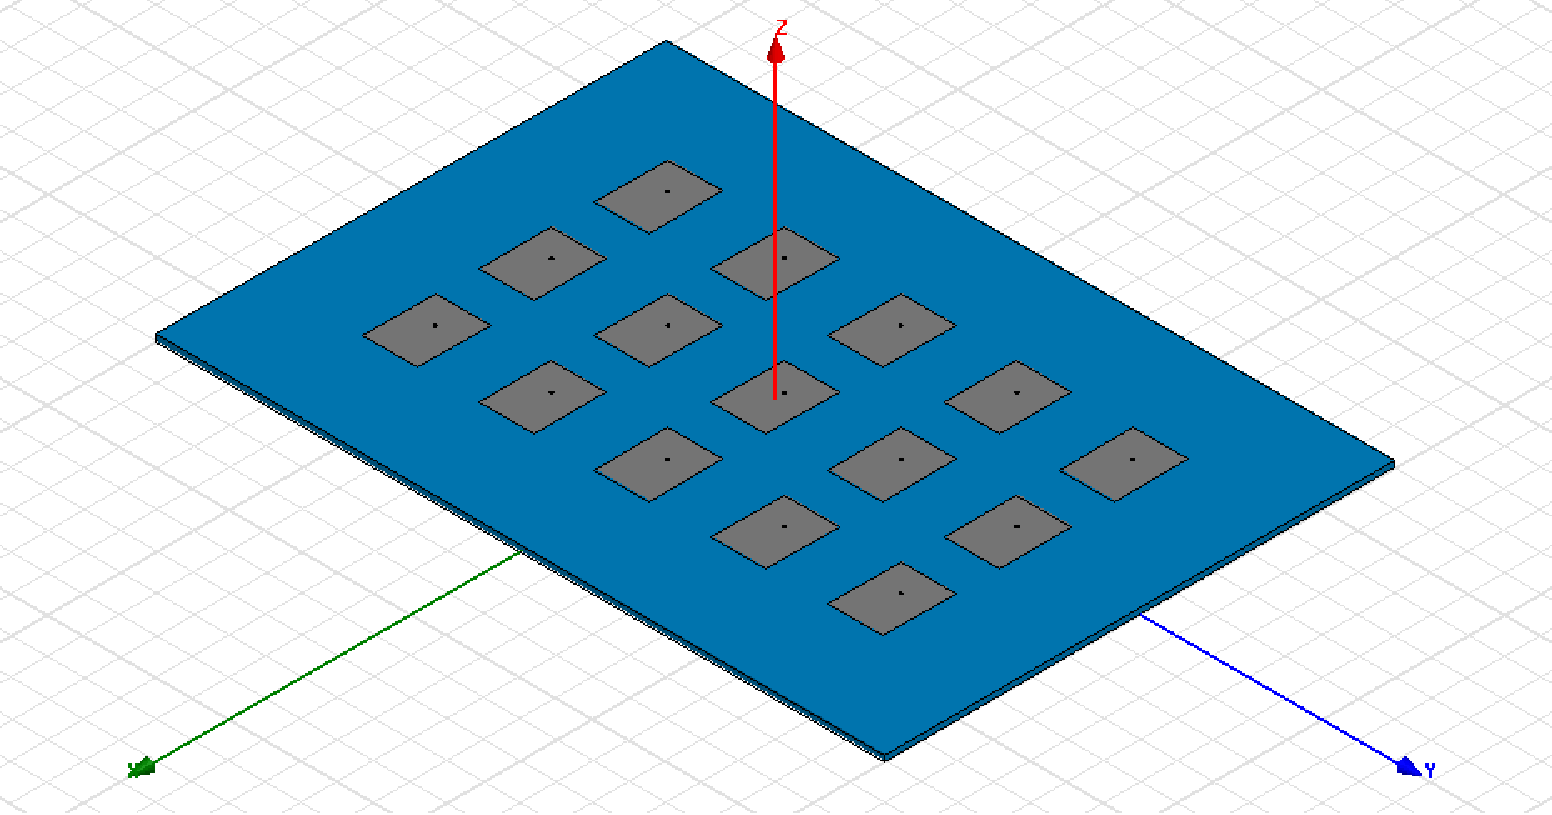
\includegraphics[width=14cm]{HFSS3x5array} 
\caption{3 by 5 patch antennas array fed by coaxial probes.}
\label{fig:HFSS3x5array}
\end{figure}

Figure \ref{fig:HFSS3x5array} shows an array of 3 by 5 patch antennas, equally spaced of $\nicefrac{\lambda_0}{2}$, fed by 15 ($g$) individual coaxial wave ports. The metal materials, that is the ground plane, the patches, an the coaxial lines and probes \cite{MilliganMAD} are set to be \itt{perfect electrical conductors} (PECs). The coaxial dielectric, necessary to hold the core of the waveguide, is made of \itt{Teflon} with $\epsilon_r = 2.1$ and its \itt{dielectric loss tangent} is of $\delta = 0.001$. The dielectric substrate of the patches is of \itt{Rogers RT/duroid 5880}, which has an $\epsilon_r = 2.2$ and a $\mrm{tan}\delta = 0.0009$. The patches have been designed in order to be resonant at 2.35 GHz. The triangulated mesh, performed by the $h$-adaptive solver of HFSS, for a minimum $\Delta S = 0.12$ (scattering parameters at the ports) between two consecutive adaptive steps is shown in figures \ref{fig:HFSS3x5Mesh} and \ref{fig:HFSS3x5MeshFull}. The basis chosen are first order polynomials and the maximum tetrahedra dimension $h = \nicefrac{\lambda}{3}$ (not $\nicefrac{\lambda_0}{3}$, as in the dielectric media the wavelength is shorter). The total computation time have been of about 58 minutes on a dual core, 2 GHz machine, with a maximum physical memory requirement of 1.5 GB.
\begin{figure}[hbpt!]
\centering

\includegraphics[width=14cm]{HFSS3x5Mesh} 
\caption{Resulting mesh of the 3 by 5 patch antennas array.}
\label{fig:HFSS3x5Mesh}
\end{figure}
\begin{figure}[hbpt!]
\centering
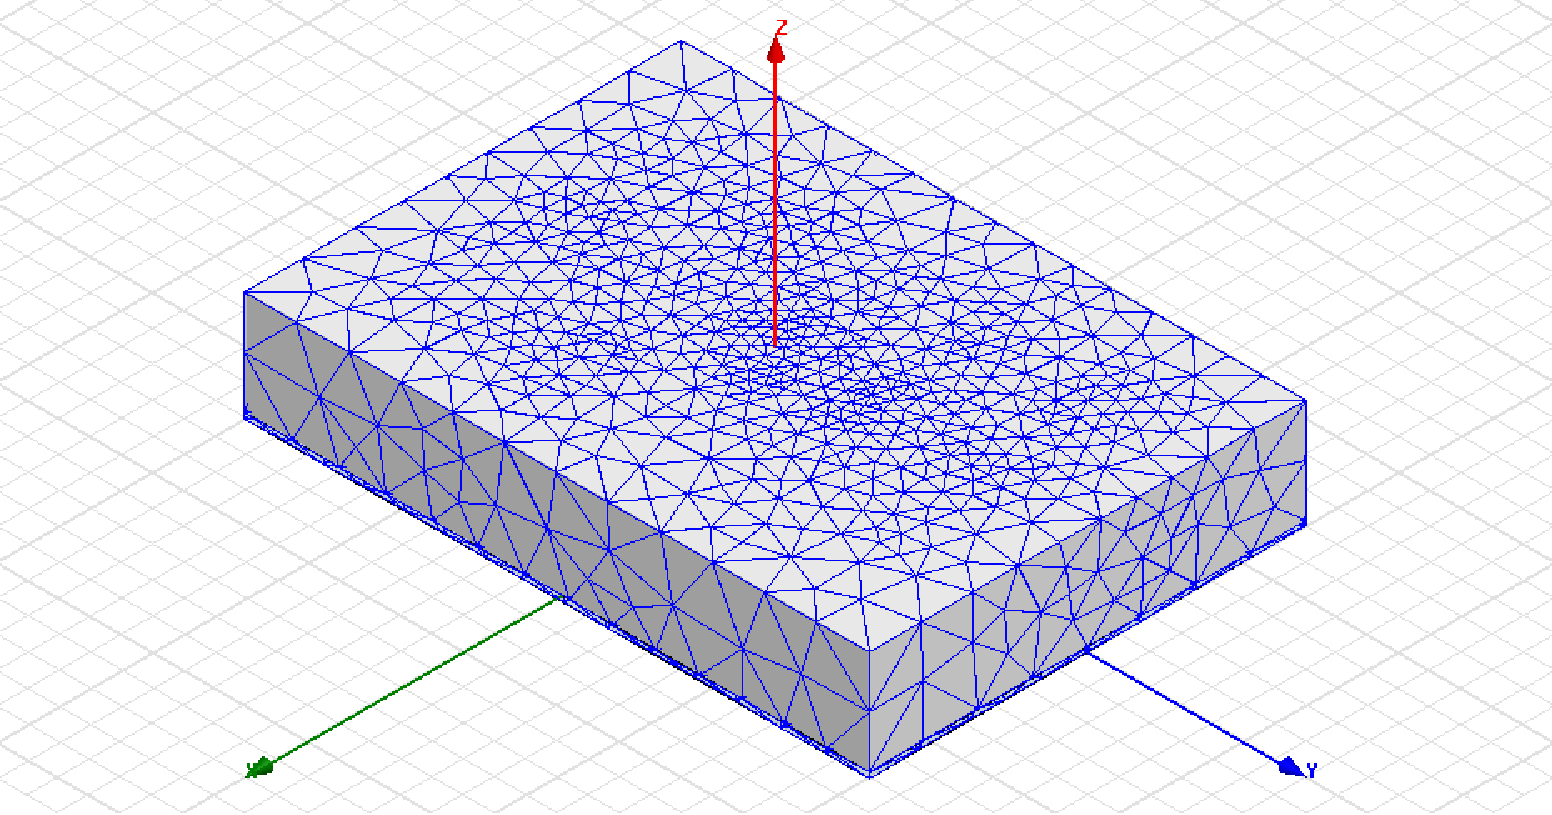
\includegraphics[width=14cm]{HFSS3x5MeshFull} 
\caption{Resulting bounding box mesh of the 3 by 5 patch antennas array.}
\label{fig:HFSS3x5MeshFull}
\end{figure}

\par From these physical data, it has been possible to build the input system matrices of our model. Using the same interpolation basis, the resulting number of unknowns has been of 358 648. The total time required to build the full model is of about 45 minutes, and most of the time is used to build $\mat F$ and the solutions of the input system matrix. Before we proceed generating the output system matrices, we must select the sampling points within the FEM domain. The sampling resolution we have chosen is of $\approx \nicefrac{\lambda_0}{10}$, with $\lambda_0 = 12.76 \ \mrm{cm}$ at 2.35 GHz. As we have seen in section \ref{sec:NumResChap1}, such a sampling resolution provides an error of about $\varepsilonup_{[\nicefrac{\lambda}{10}]} \approx 2 \ 10^{-3}$, which is adequate for our patterns computations. Further errors are introduced by the sampling operation in a FEM domain. In effect, the field within the discretized domain suffers of discontinuities at the interfaces between the elements, especially if the fields that are approximated vary rapidly. The $h$-adaptive meshing reduces this undesired behavior, but cannot eradicate it completely. Thus for better accuracy, a volume interpolation should be performed as proposed in \cite{MonkN2F}, where the surface integrals are achieved through volume integrals within a thin layer that contains the fields sampling points. Also, the finite element method suffers of numerical dispersion in electrically large electromagnetic models \cite{IhlenburgBabuskaDAEE}, especially for high $h$ (tetrahedra dimension) and low $p$ (polynomial order). In our approach, we will consider these errors to be absent, remembering that they involve both the full and the reduced order models, and a comparison between these two models is unaffected by such errors. The near fields sampling grid is shown in figure \ref{fig:HFSS3x5arraySMPL}.
\begin{figure}[hbpt!]
\centering
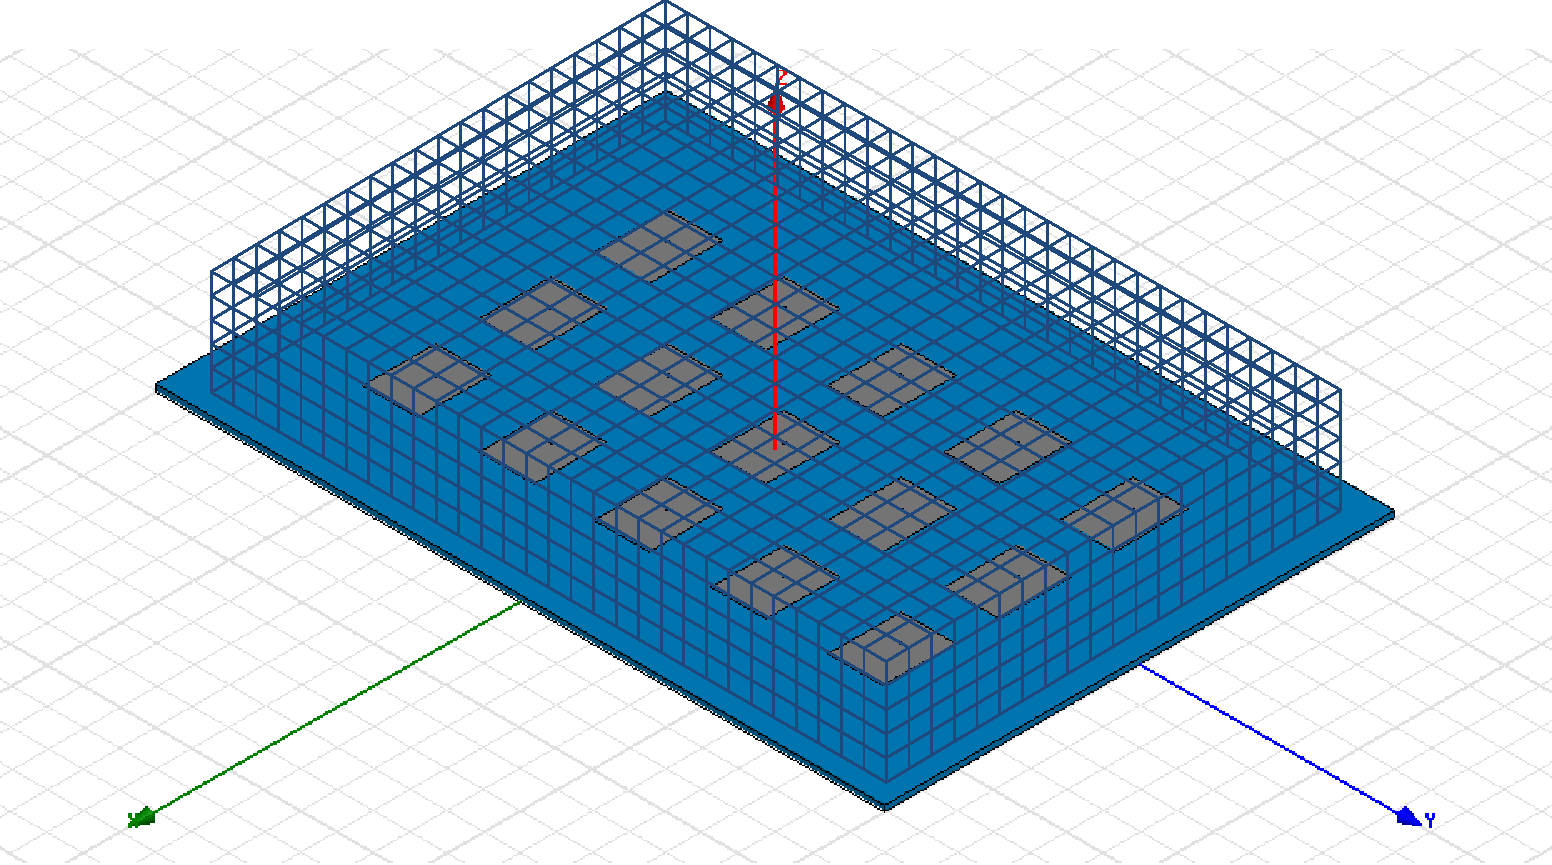
\includegraphics[width=14cm]{HFSS3x5arraySMPL} 
\caption{Sampling grid on the 3 by 5 patch antennas array.}
\label{fig:HFSS3x5arraySMPL}
\end{figure} The ABCs are located $\approx 0.6 {\lambda_0}$ from the center of the patches and the sampling grid at $\approx \nicefrac{\lambda_0}{2}$. The bottom face of the parallelepiped have been neglected, as the fields on the PEC ground plane are known to be null. The directivity pattern computed by HFSS is shown in figure \ref{fig:HFSS3x5pattern}.
\begin{figure}[hbpt!]
\centering
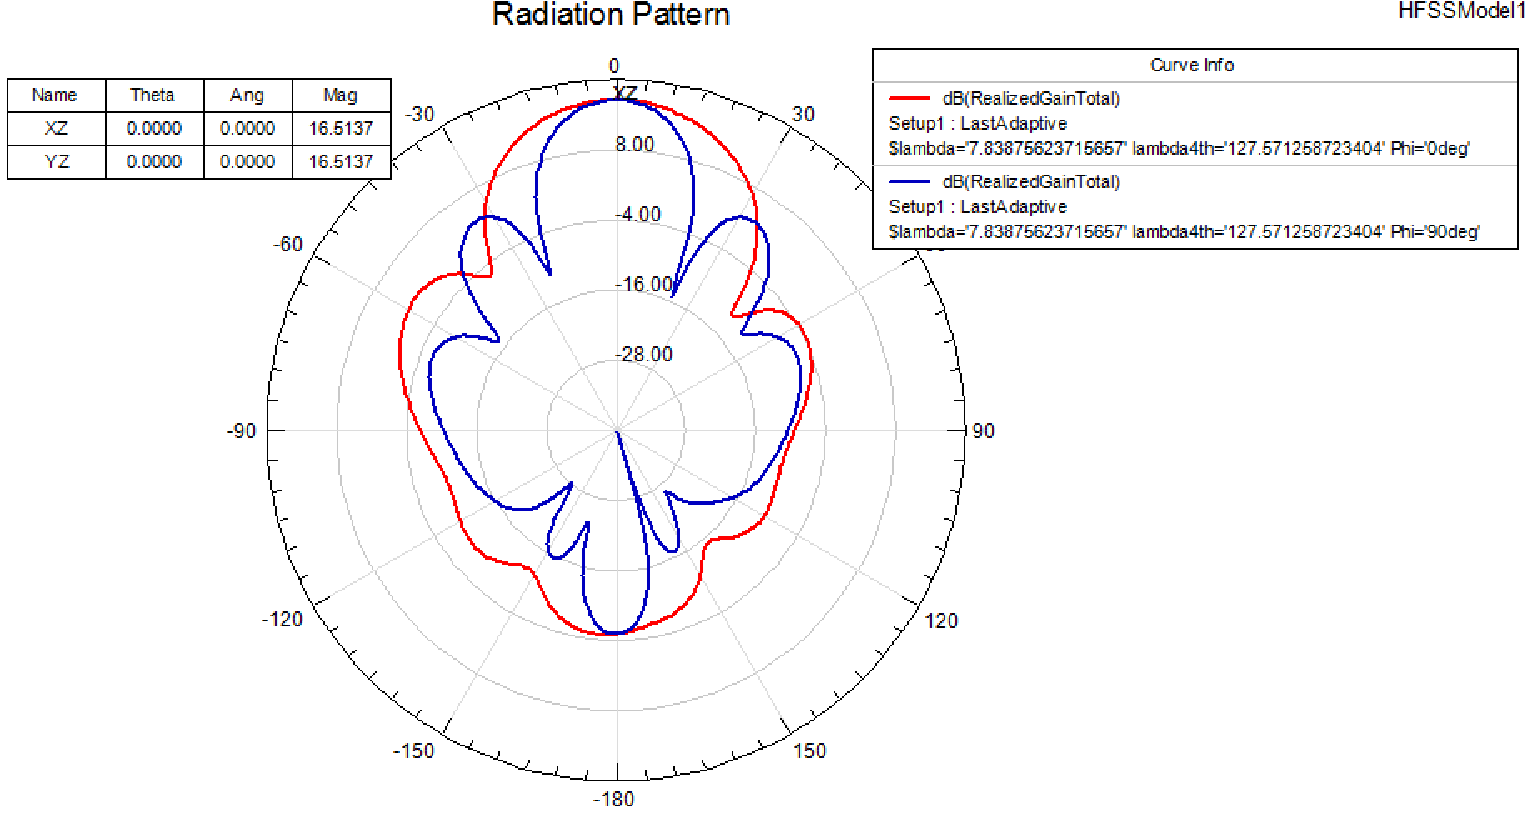
\includegraphics[width=14cm]{HFSS3x5pattern} 
\caption{Broadside directivity pattern of the 3 by 5 patch antennas array computed by HFSS.}
\label{fig:HFSS3x5pattern}
\end{figure} The output system matrices, according to the results of figure \ref{fig:errorDFT_5}, can be built with a DFT-truncation retaining only 21 coefficients. Hence, we obtain an output matrix $\colspan{\mat{c}{'}_j} \in \mathbb{C}^{358 648 \times 21}, 1 \leq j \leq 21$ for each polarization, and the planes of pattern computation will be the XZ and YZ cut planes. This completes our radiation model. The total memory employed, considering double precision, is detailed in table \ref{tab:memFull}.
\begin{table}[!tbp]
\centering
\begin{tabular}{|c|c|}
\hline Matrix & Memory [Bytes]\\
\hline \hline
$\mat A$ & 109 231 240 \\
$\spanning{\mat{b}_1, \ldots, \mat{b}_{15}} $ & 488 \\
$\spanning{\mat{x}_1, \ldots, \mat{x}_{15}}$ & 86 075 520 \\
XZ plane : $\spanning{\mat{c}{'}_1, \ldots, \mat{c}{'}_{21}}_\mrm{\theta} + \spanning{\mat{c}{'}_1, \ldots, \mat{c}{'}_{21}}_\mrm{\phi}$ & 9 037 568 \\
YZ plane : $\spanning{\mat{c}{'}_1, \ldots, \mat{c}{'}_{21}}_\mrm{\theta} + \spanning{\mat{c}{'}_1, \ldots, \mat{c}{'}_{21}}_\mrm{\phi}$ & 9 037 568 \\
\hline Total & $\approx 221$MB \\
\hline
\end{tabular}
\caption{Memory requirements for the full radiation model.}
\label{tab:memFull}
\end{table} As most of the matrices are sparse, the only real contributions are given by the FEM system matrix and the solution vectors which are not sparse. Thanks to the DFT truncation and to the few number of sampling points (1100), the output system matrix is very low memory consuming, and building a matrix of trigonometric polynomials sampled values in order to compute the pattern on 5000 look angles within $[0\�, 360\�)$ requires only 1.6 MB more. Notice that this matrix is the same for all the planes, thus has to be computed only once.

\par We can now build our reduced order model. Before we proceed with Galerkin projection method, we may discuss on the array configuration and how should be the near fields scanning space. According to the results of section \ref{sec:approxNF}, the rank for a scanning along the $x$ direction, as we have 3 patches spaced of $\nicefrac{\lambda_0}{2}$, should be of 3. Analogously, along the $y$ direction, as we have 5 patches spaced of $\nicefrac{\lambda_0}{2}$, the rank should be of 5. Thus, until we use 3 or 5 solutions pictures, for a beam steering operation in each respective cut-plane, we expect the error to be non negligible.

\par To check the functionality of the ROM, we have performed a Galerkin projection selecting as scan angle the broadside direction. The resulting directivity pattern is shown in figure \ref{fig:patchPatternBS}.
\begin{figure}[hbpt!]
\centering
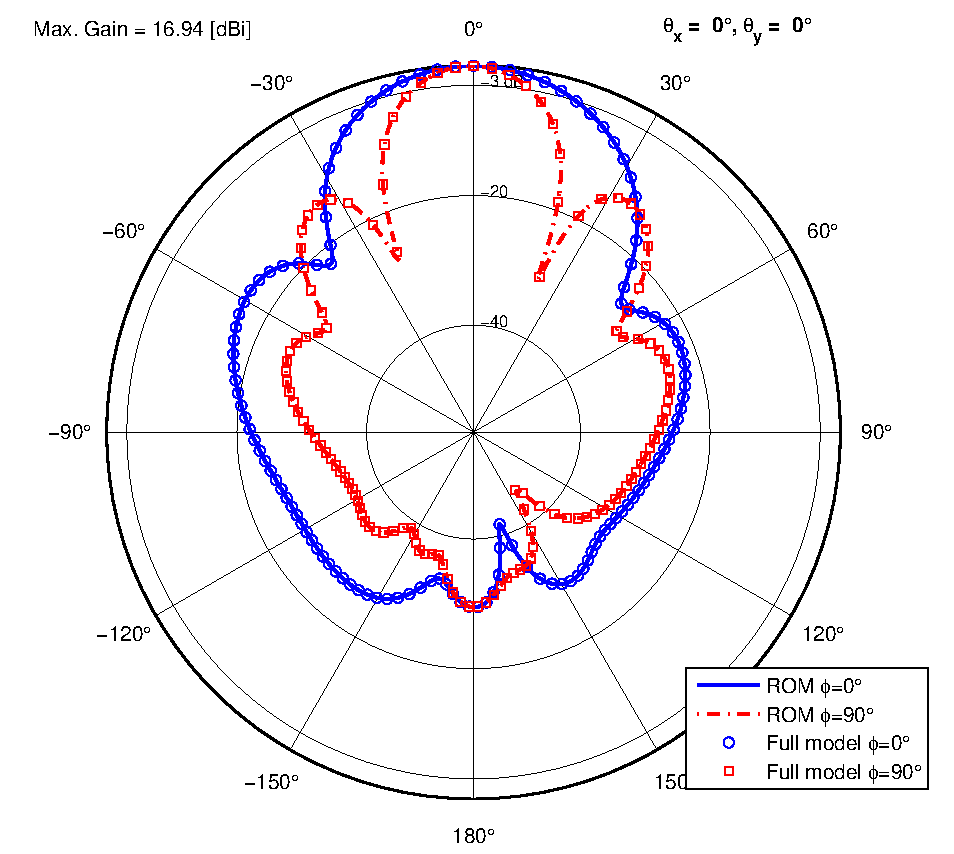
\includegraphics[width=12cm]{patchPatternBS} 
\caption{Total far fields directivity pattern computed in the broadside direction by the full model and the ROM of the 3 by 5 patch antennas array.}
\label{fig:patchPatternBS}
\end{figure} The total relative error introduced by the model order reduction is numerically null ($3.395 \ 10^{-13}$). There are some differences between the pattern computed by HFSS and ours. This is mainly due to the fact the our sampling points are distant form the radiation boundaries from which HFSS computes the far fields patterns. In effect, as we chose sampling points slightly distant from the radiation boundaries (1mm close to the surface), we notice a higher similitude of our pattern with HFSS's one, as shown in figure \ref{fig:patchPatternBSnearABC}.
\begin{figure}[hbpt!]
\centering
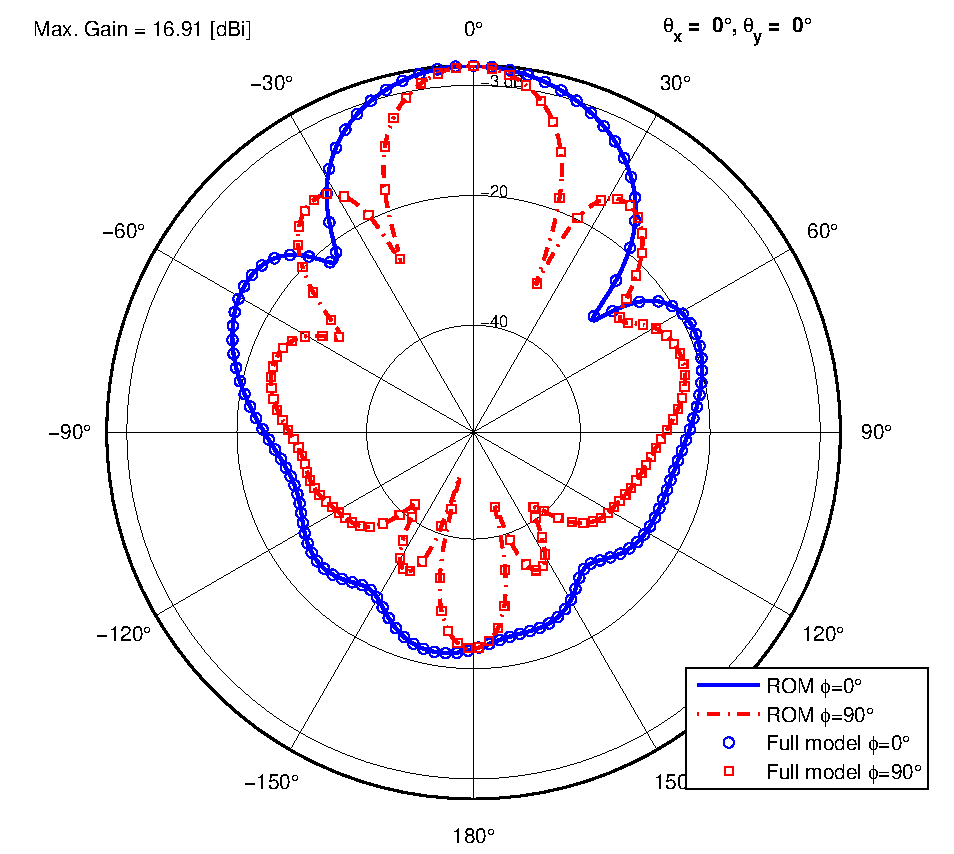
\includegraphics[width=12cm]{patchPatternBSnearABC} 
\caption{Broadside directivity pattern computed from a surface 1mm next to the radiation boundaries.}
\label{fig:patchPatternBSnearABC}
\end{figure} However, the main purpose of this thesis is to discuss the application of the projection-based model order reductions on phased arrays, with an emphasis on the reduced order dimension. Hence, we proceed working on the first near fields sampling points selection, without carrying on whether HFSS or our implementation is more accurate. % Our hypothesis on the accuracy is that the arbitrary imposition of the wave impedance to $\zeta_0$ (ABCs) leads to high errors the radiating structure being electrically large, and the minimum distance of the radiation boundaries should be of $\frac{2 \ \mrm{L}^2}{\lambda}$ (see note \ref{fn:NF2FFdist}). Thus the computation of the electric and magnetic fields, related by the real wave impedance (with previously discussed numerical errors), may lead to a better accuracy of the pattern.

\subsubsection{Galerkin projection method on cut planes}

\par We have chosen the beam steering angles to be along the $y$ direction in which we have 5 groups of 3 antennas excited with a linear phase, each group having the same phase. The spanning scan angles are chosen equidistant in the range of $\theta_y \in [0\�,90\�]$. Then the error is computed for 21 tested scan angles chosen in the same range, returning for each spanning space dimension the average relative error between the full model and the MOR computed far fields detectors on both XZ and YZ planes. The results are shown in figure \ref{fig:spanErrorAvg}.
\begin{figure}[hbpt!]
\centering
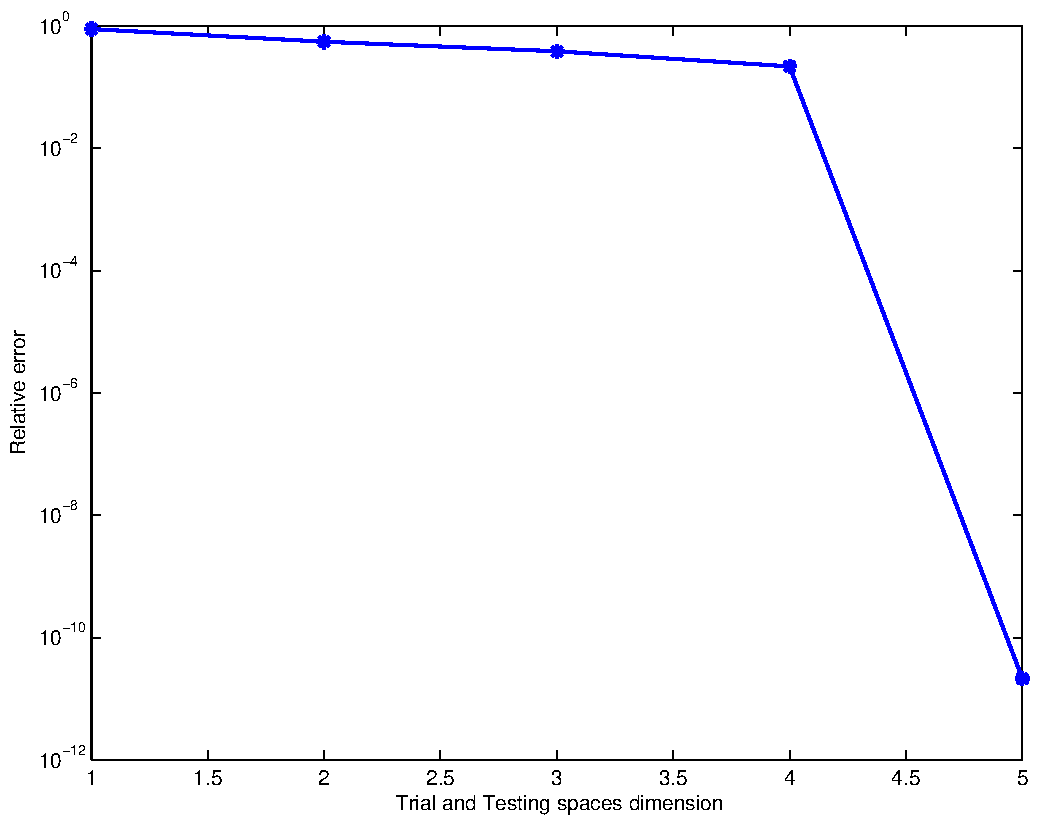
\includegraphics[width=10cm]{spanErrorAvg} 
\caption{Relative error in the far fields detectors for the full model and those for the reduced model.}
\label{fig:spanErrorAvg}
\end{figure} The average error value computed with a scan angle space of dimension 4 is of $0.2189$. This is still to high for accurate computations, and a steered patterns in that conditions are shown in figures \ref{fig:patchPatternnextBS} and \ref{fig:patchPatternnextEF}.
\begin{figure}[!hbtp]
\begin{minipage}[b]{0.5\linewidth} % A minipage that covers half the page
\centering
\includegraphics[width=7.3cm]{patchPatternnextBS}
\caption{Steered pattern close to broad side computed from a ROM of order 4.}
\label{fig:patchPatternnextBS}
\end{minipage}
\hspace{0.1cm} % To get a little bit of space between the figures
\begin{minipage}[b]{0.5\linewidth}
\centering
\includegraphics[width=7.3cm]{patchPatternnextEF}
\caption{Steered pattern close to end fire computed from a ROM of order 4.}
\label{fig:patchPatternnextEF}
\end{minipage}
\end{figure} As we expected from conclusion \ref{cc:BSEFselectionSpace}, the pattern next to end fire is more accurate than that close to broadside. Furthermore, this behavior should be enhanced by the element factor allowing us to choose spanning angles much closer to the broadside direction. Now, we conclude discussing on the error we obtain with the ROM of order 5: it is null for all steering  angles chosen along the $y$ direction. This is the most interesting information achieved from the model order reduction of phased arrays. The final model is constituted of the following full (not sparse) matrices : $\tilde \mat A \in \mathbb{C}^{5 \times 5}$, $\colspan{\tilde{\mat{b}}_1, \ldots, \tilde{\mat{b}}_{15}} \in \mathbb{C}^{5 \times 15}$, $\colspan{\tilde{\mat{c}}{'}_1, \ldots, \tilde{\mat{c}}{'}_{21}}_\theta, \colspan{\tilde{\mat{c}}{'}_1, \ldots, \tilde{\mat{c}}{'}_{21}}_\phi \in \mathbb{C}^{5 \times 21}$ for each cut-plane, and $\tilde \mat F \in \mathbb{C}^{1100 \times 5}$, necessary in order to compute the radiated power from $p = 1100$ near fields sampling points. 420 kB are occupied by this ROM, and we only need to supply the scan angles $\Theta_i(0\�, \theta_y)$ and the output trigonometric polynomials values $\Omega_j (\theta, \phi=0\�, 90\�)$, the latter depending on the required pattern resolution (we used a $\Delta \theta$ of 0.036\� building a matrix of about 1.6 MB in this case), to compute the cut-planes patterns. The error is now pending on the sampling resolution of $\nicefrac{\lambda}{10}$, which has been considered to provide accurate patterns.


\subsubsection{Dual space projection method on cut planes}

\par We proceed illustrating the effectiveness of the dual problem based projections. We need to compute further 21 solutions from the output vectors we dispose. We have chosen to match the look angles in the $\theta$ polarization, using the output matrix $\colspan{{\mat{c}}{'}_1, \ldots, {\mat{c}}{'}_{21}}_\theta$, with matching look angles in 89.7297\�, 179.8198\� and 269.9099\� and the test space is matched in 0\�, 45\� and 90\� to build a ROM of order 3. As 11\� is not an interpolation angle for both the test and trial spaces, we use that scan angle to compute the error.
\begin{figure}[hbpt!]
\centering
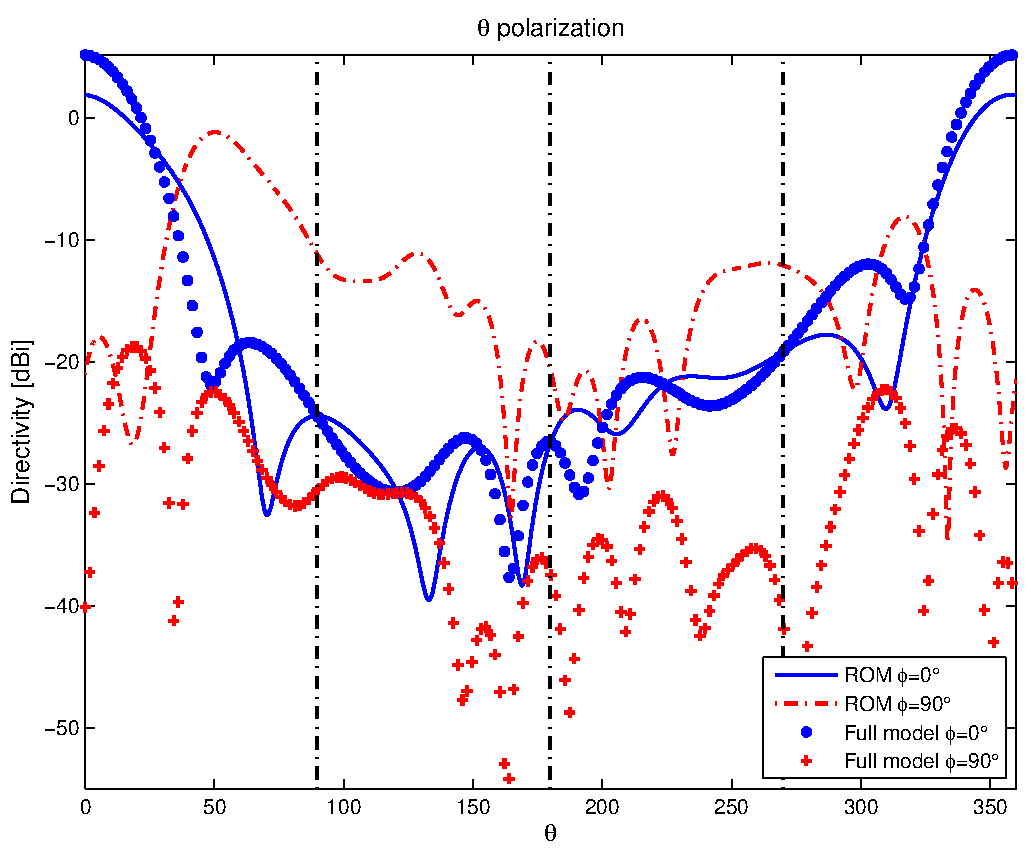
\includegraphics[width=12cm]{dual3theta} 
\caption{$\theta$ polarization pattern for the full model and those for the reduced model of order 3 with look angle trial space.}
\label{fig:dual3theta}
\end{figure}
\begin{figure}[hbpt!]
\centering
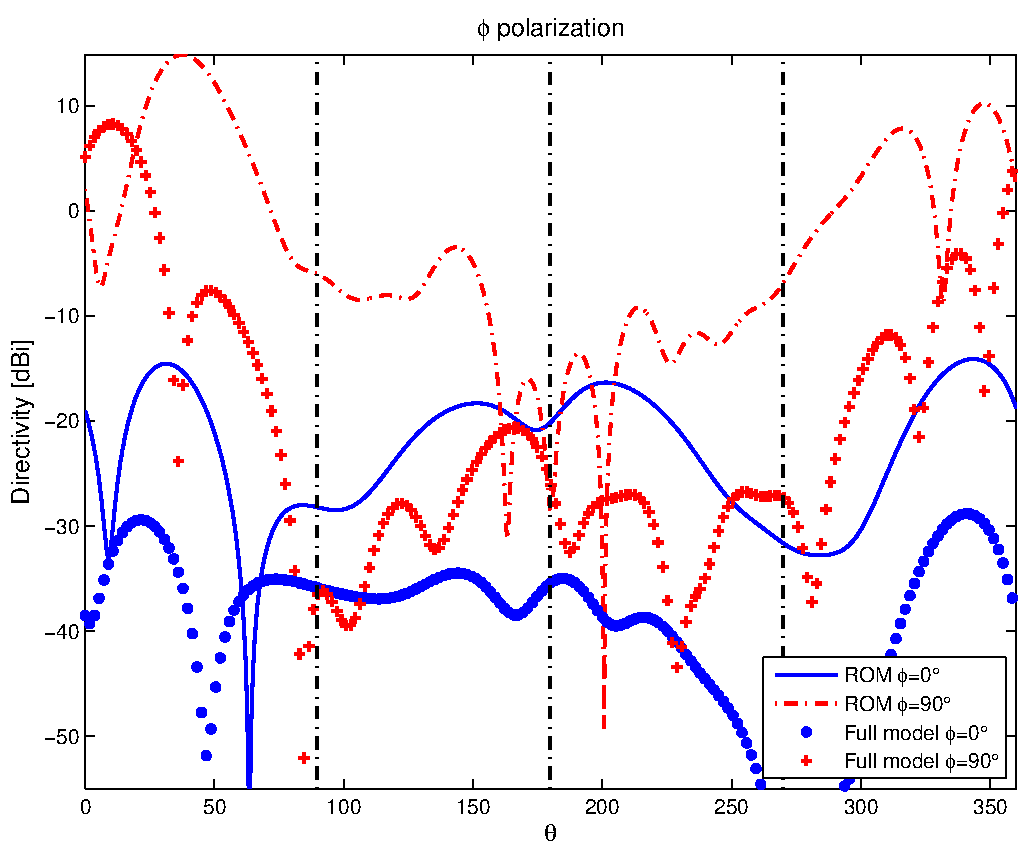
\includegraphics[width=12cm]{dual3phi} 
\caption{$\phi$ polarization pattern for the full model and those for the reduced model of order 3 with look angle trial space.}
\label{fig:dual3phi}
\end{figure}
Figures \ref{fig:dual3theta} and \ref{fig:dual3phi} show that the pattern is matched (null error) in the look angles selected for the trial space in the XZ plane (dash-dotted vertical lines) only for the $\theta$ polarization on the XZ plane, while the whole pattern error remains very high as the 3 spanning vectors of the trial space do not constitute a basis. We achieve only a local matching on the selected look angles and this is a result we could expect from the definition of the look angle. While the scan angle contains informations on the whole near fields on the bounding surface, the look angle, being the result of a near-to-far transformation, does not maintain any information on the near fields, hence on the total pattern. Furthermore, as the trial and the test spaces must have equal dimensions to allow the inversion of $\tilde \mat A$ during the solution of the reduced order input system, it will never be possible to cover the entire pattern matching the look angle space. Another non negligible negative point is associated to the fact that the number of coefficients retained with the DFT-truncation, considering all the polarizations and all the cut-planes, is typically higher than the number of scan angles that span the trial space, leading in further computations that may not improve the accuracy.

\subsubsection{Galerkin projections for three-dimensional scanning}

\par It is our interest to see now whether the ROM behaves if we want to scan the whole three-dimensional space. In a first attempt, we build the scan angle spaces from scan angles in both $x$ and $y$ directions, that is with 3 angles $(\theta_x, \theta_y = 0\�)$ and 5 angles in $(\theta_x = 0\�, \theta_y)$, with $\theta_x, \theta_y \in [0\�, 90\�]$. The 8 selected angles, chosen properly in order to avoid the redundancy in the broadside direction, and the tested scan angles in the $\phi = 45\�$ are shown in figure \ref{fig:sel3x5angles}.
\begin{figure}[hbpt!]
\centering
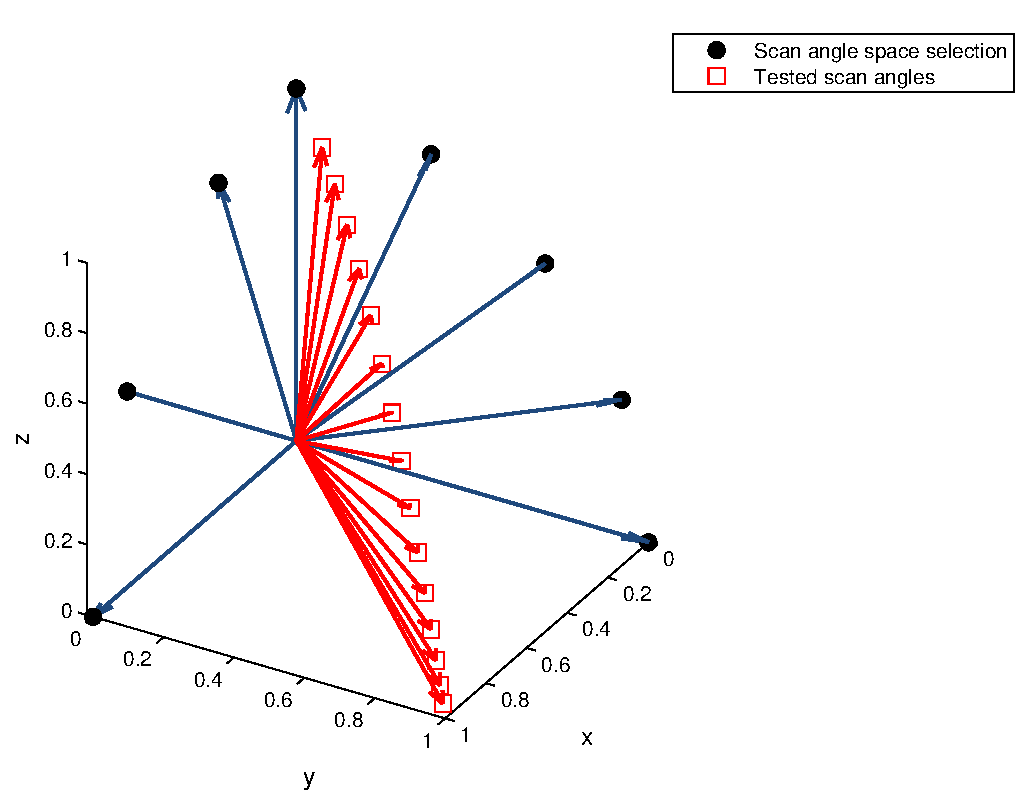
\includegraphics[width=12cm]{sel3x5angles} 
\caption{Scan angle selected for the projection space and tested angles (unit vectors of the directions).}
\label{fig:sel3x5angles}
\end{figure} The resulting error, illustrated in figure \ref{fig:linCombError}, shows that we cannot consider the oblique scan angles as a linear combination of the space spanned by scan angles in the $x$ and $y$ beam steering directions: the error never drops below $10^{-2}$.
\begin{figure}[hbpt!]
\centering
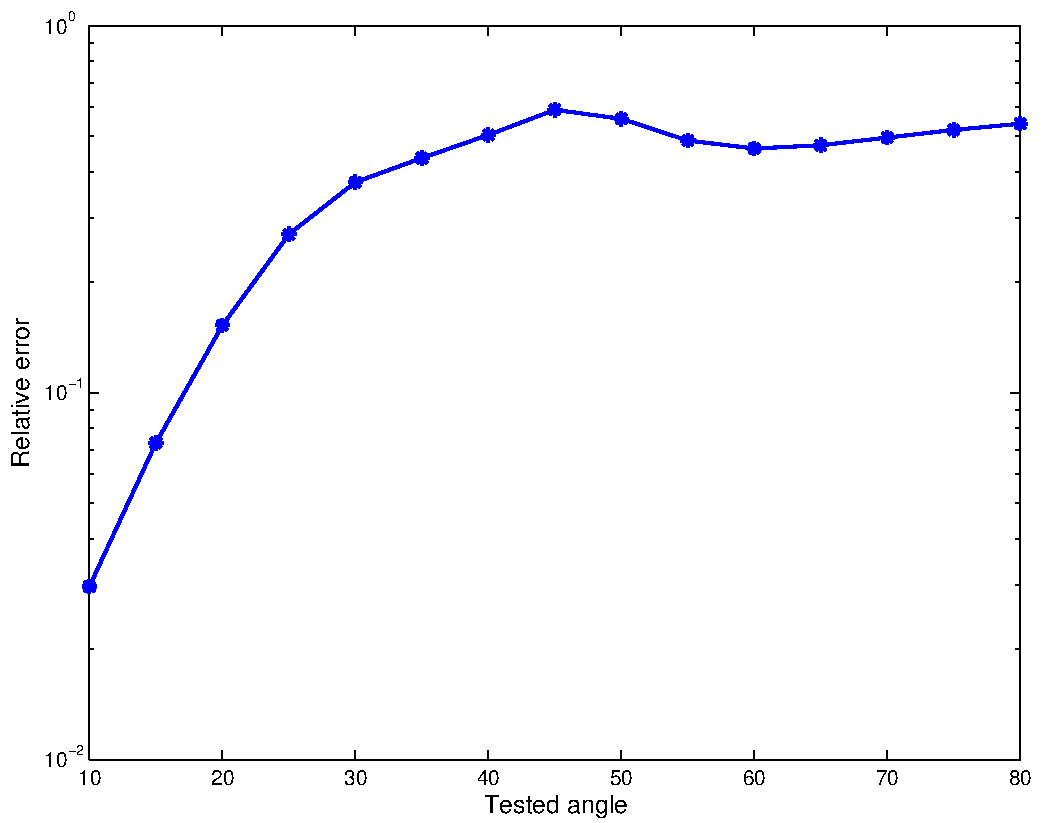
\includegraphics[width=12cm]{linCombError} 
\caption{Error resulting from an oblique scan angle testing.}
\label{fig:linCombError}
\end{figure} 

\par From this results we understand that we need to select more vectors, with scan angles in the entire septentrional hemisphere. The first idea that comes to our minds is to employ a spiraling helicoidal trajectory to select the scan angles for the test space and an opposite one to test the quality of the space spanned. Those trajectories are depicted in figure \ref{fig:spirHeltraj}.
\begin{figure}[hbpt!]
\centering
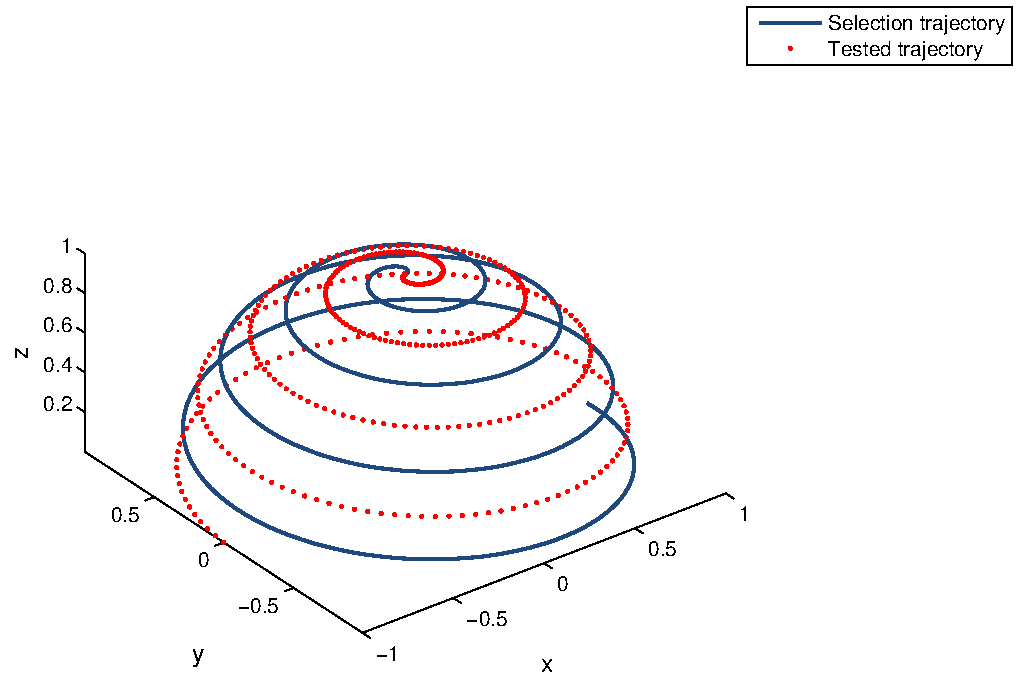
\includegraphics[width=12cm]{spirHeltraj} 
\caption{Scan angles selection trajectory and error test scan angles trajectory.}
\label{fig:spirHeltraj}
\end{figure}
We proceed computing the errors increasing the size of the scan angle space, the results are shown in figure \ref{fig:spirHelErrorSVD}
\begin{figure}[hbpt!]
\centering
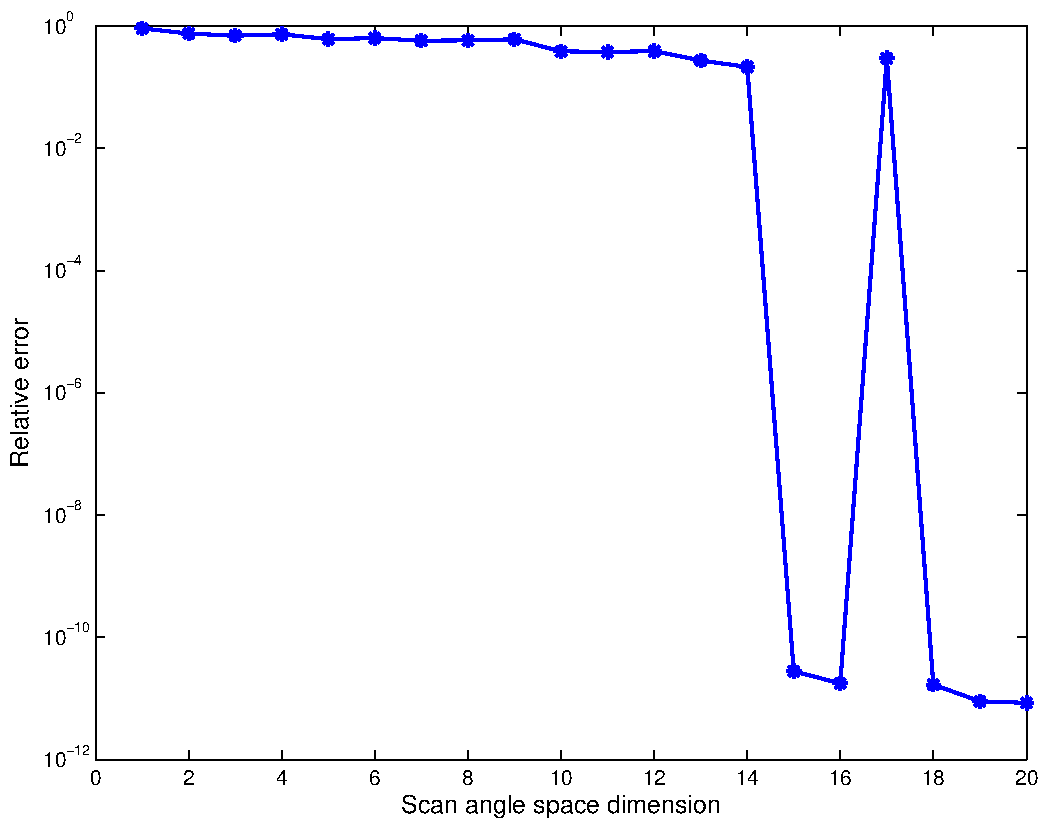
\includegraphics[width=12cm]{spirHelErrorSVD} 
\caption{Average error on the test scan angles patterns with a space spanned with a spiraling helicoidal trajectory.}
\label{fig:spirHelErrorSVD}
\end{figure} First we notice that the error becomes numerically null at 15 scan angles on the selection trajectory, that is the total number of array antennas. The error suddenly becomes non null with 17 scan angles. This is mainly due, as we can see in figure \ref{fig:spirHeltraj17}, to the spherical pyramid edge sampling condition we have achieved with 17 scan angles. The resulting vectors are linearly dependent, located only along the $x$ and $y$ directions, hence the full rank of 15 is not attained.
\begin{figure}[hbpt!]
\centering
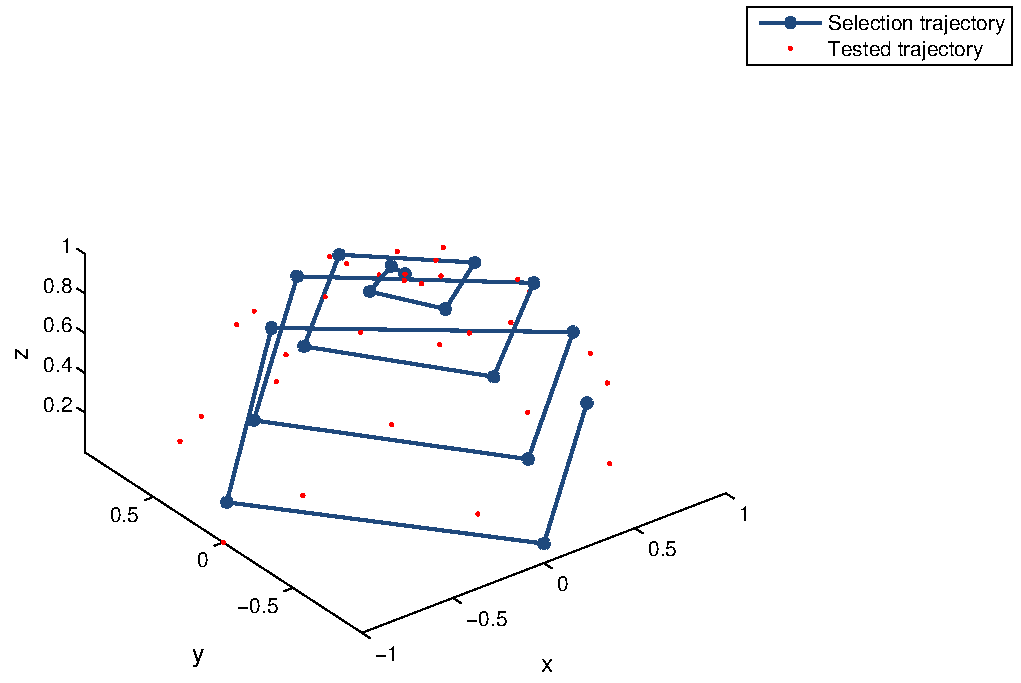
\includegraphics[width=12cm]{spirHeltraj17} 
\caption{17 scan angles selection trajectory and 31 error test scan angles trajectory.}
\label{fig:spirHeltraj17}
\end{figure} We can conclude that
\begin{mycc}
The number of scan angles required in order to correctly approximate a three-dimensional steering operation all over an hemisphere, for $\nicefrac{\lambda}{2}$ spaced array elements, is of the total number of radiating array elements. Furthermore, the scan angles must be chosen properly, in order to obtain a set of linearly independent vectors. These can be selected along a spiraling helicoidal trajectory over the septentrional hemisphere of a sphere aligned with the center of the array.
\end{mycc}

\par Finally, we can compute the radiation solid with the ROM of order 15. To scan the whole space, we have chosen cut-planes in the range $\phi \in [0\�,180\�)$ with a $\Delta \phi \approx 3\�$, while the sampled trigonometric polynomials matrix $\mat t$ covers the range $[0\�, 360\�)$. The total ROM occupies only 3.2 MB of memory, and each new scan angle pattern is computed with the sampling resolution accuracy of $\approx 2 \ 10^{-3}$ in about 0.07 seconds on a dual core 2 GHz machine, while the full model requires 0.55 seconds for each scan angle.

\begin{figure}[hbpt!]
\centering
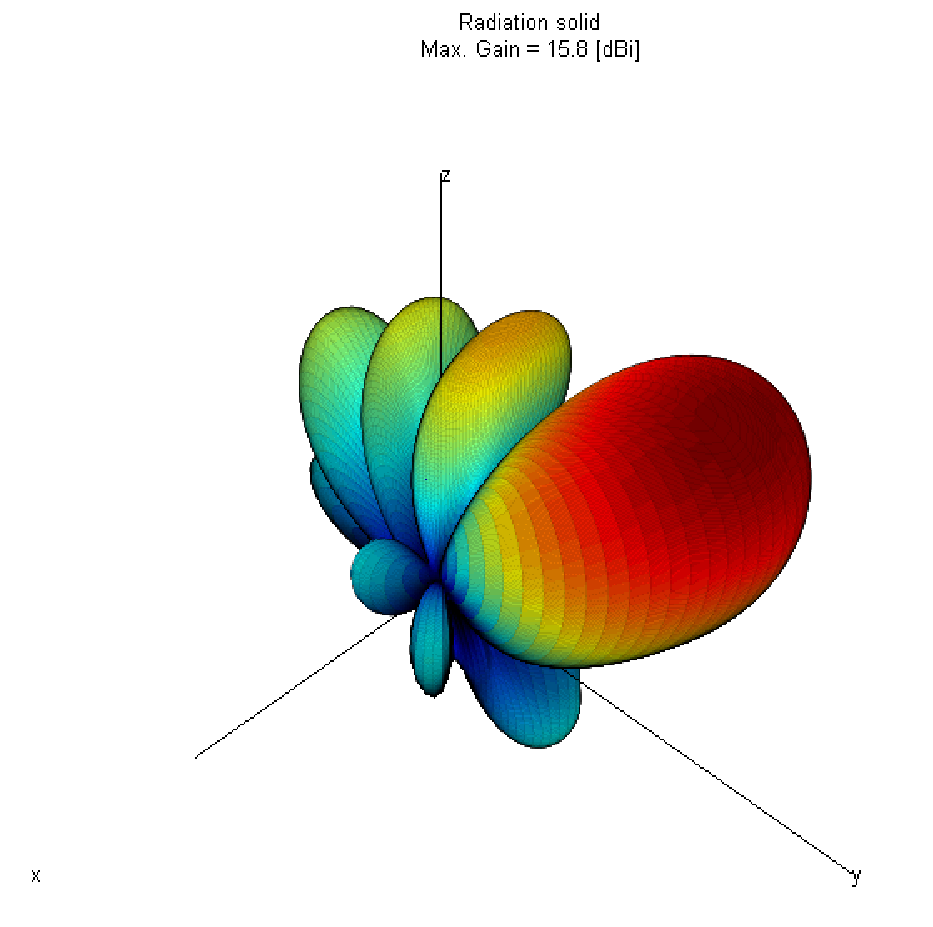
\includegraphics[width=14cm]{RadSolid} 
\caption{Radiation directivity pattern scanning in $(\theta_x=-10\�, \theta_y=45\�)$ computed by the reduced order model.}
\label{fig:RadSolid}
\end{figure}


\subsection{40 dual-polarized tapered slot antennas} 

\par To emphasize the importance of the relative spacing between the radiating elements, we now illustrate the results of the model order reduction applied to the array of in figure \ref{fig:TSA}.
\begin{figure}[bpt!]
\centering

\includegraphics[width=14cm]{TSA} 
\caption{Array of tapered slot antennas equally spaced of $\approx \nicefrac{\lambda_0}{5}$.}
\label{fig:TSA}
\end{figure} It is a dual polarized array of 40 tapered slot antennas (TSAs), also called \itt{Vivaldi} antennas, that is actually built superposing orthogonally two arrays (each ideally linearly polarized) of 4 by 5 of TSAs. The model has been designed according to \cite{ChioSchaubertPSDWB}. Notice that in figure \ref{fig:TSA}, the front $x$ directed row of TSAs have some dielectrics parts hidden in order to show the feeding stripline, with radial stub termination. The radiating slots are tapered exponentially, while short circuited at the non radiating side. With the given geometrical parameters, the TSA achieves a bandwidth, in terms of \itt{Voltage Standing Wave Ratio} (VSWR) below 2, of about 5.5 GHz when steering in the broadside direction, centered at 4 Ghz. We have chosen to build the radiation model at 3 GHz, for which the spacing between the TSAs, being of 2cm, is of $\approx \nicefrac{\lambda_0}{5}$. The near fields sampling resolution is chosen to be of $\nicefrac{\lambda_0}{10}$ and the number of coefficients retained in the DFT-truncation is of 51. To build the ROM with Galerkin projections, the steering direction chosen is $x$, where we have a maximum of 9 groups radiating elements, 5 being cross polarized. From the singular values of figure \ref{fig:singVal}, we realize that the rank of the scan angle space in that direction is of 9 (for scan angles selected equidistantly in the range $\theta_x \in [0\�,90\�]$, $\theta_y=0\�$).
\begin{figure}[hptb!]
\centering
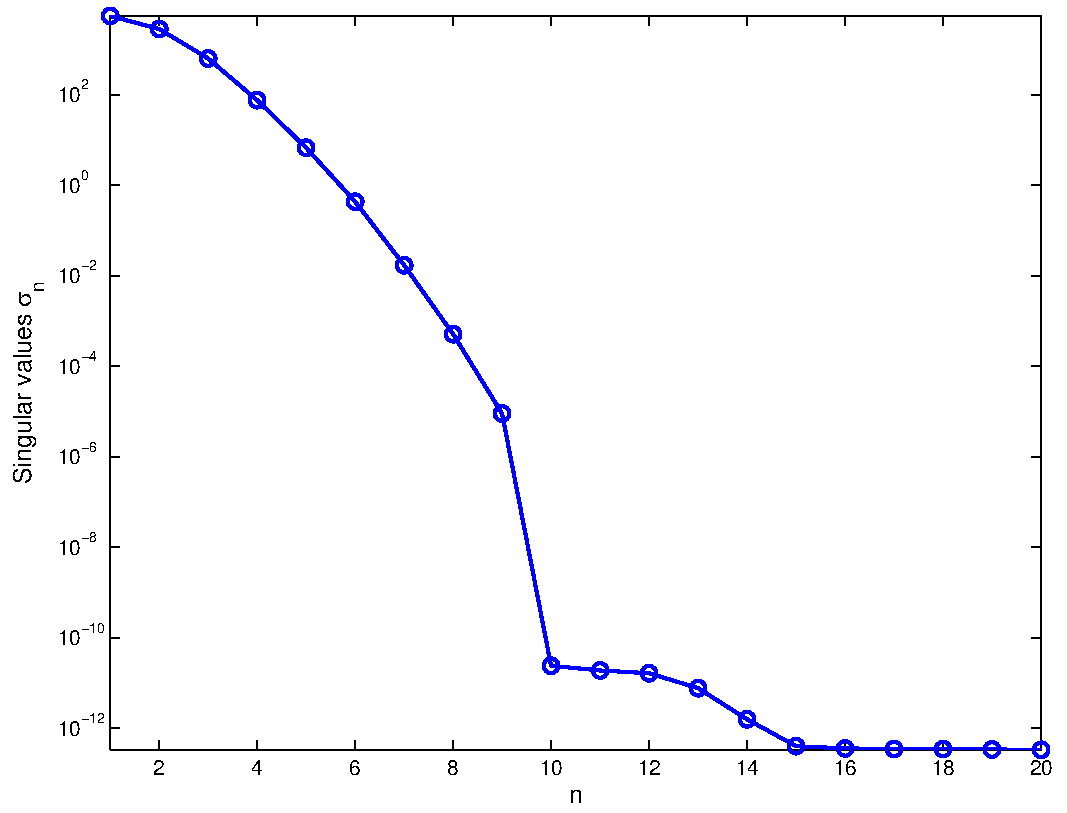
\includegraphics[width=10cm]{singVal} 
\caption{Singular values of the TSAs array steered in the $x$ direction.}
\label{fig:singVal}
\end{figure} The singular values are decreasing rapidly even before we attain the numerical rank. As we have seen in figure \ref{fig:SVDerrorExp_33_0,25}, the far fields detectors error was low even before the number of vectors arrived to the number of radiating elements. Thus we expect the ROM to require an order lower than 9 while keeping the sampling resolution error.
\begin{figure}[bpt!]
\centering
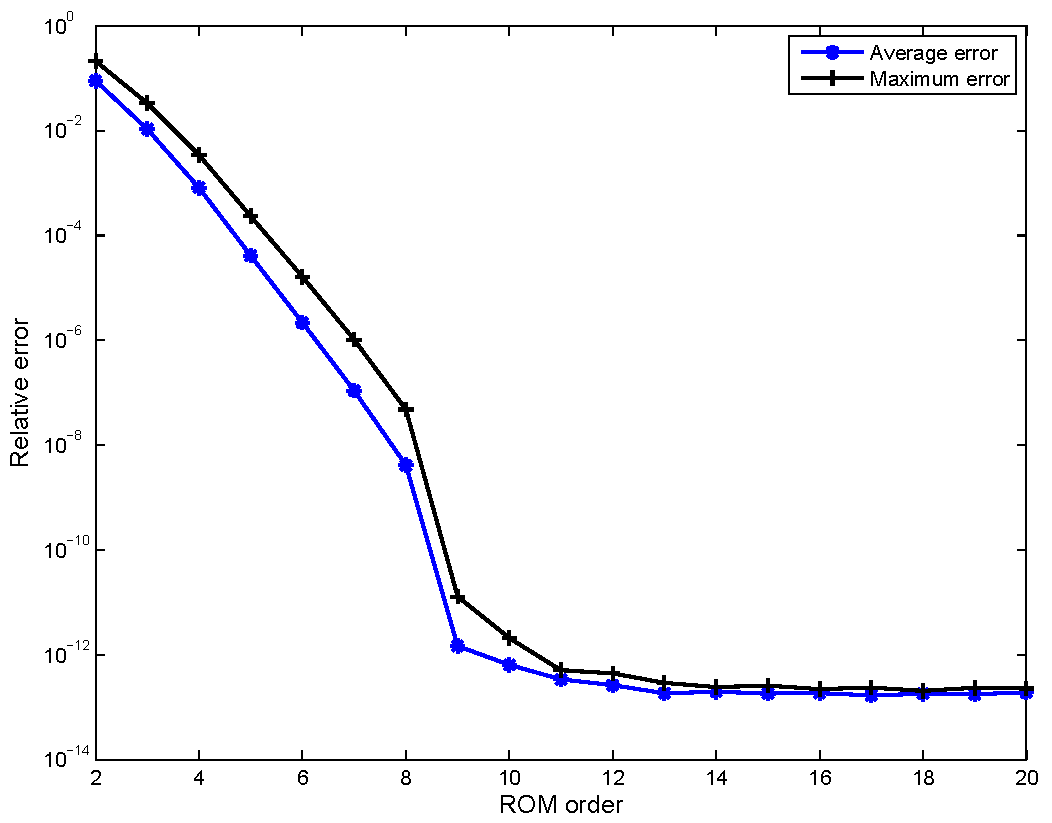
\includegraphics[width=12cm]{vivaldiError} 
\caption{Error for several orders of the TSAs array ROM.}
\label{fig:vivaldiError}
\end{figure} As we can see in figure \ref{fig:vivaldiError}, the maximum ROM approximation error, attained  near the broadside direction (figure \ref{fig:vivaldiErrorOrder5}), is slightly lower than the near fields sampling resolution error once we use 5 spanning scan angles, and using 6 out of 9 renders the approximation error irrelevant to the radiation model. 
\begin{figure}[hbpt!]
\centering
\includegraphics[width=12cm]{vivaldiErrorOrder5} 
\caption{Error introduced by a ROM of order 5 for several tested angles.}
\label{fig:vivaldiErrorOrder5}
\end{figure} Figure \ref{fig:vivaldiErrorOrder5} reports the error for several tested angles, the scan angles selected to span the projection space being of $\theta_x = 0\�, 22.5\�, 45\�, 67.5\�, 90\�$. This results in the fact we need much less than 81 spanning scan angles to scan the whole septentrional hemisphere. Figures \ref{fig:vivaldi3dError} and \ref{fig:vivaldi3dErrorZoom} show that only 40 vectors (the total number of antennas) are required to build an accurate ROM for three-dimensional beam steering of the tapered slot antennas array designed.

\begin{figure}[hbpt!]
\centering
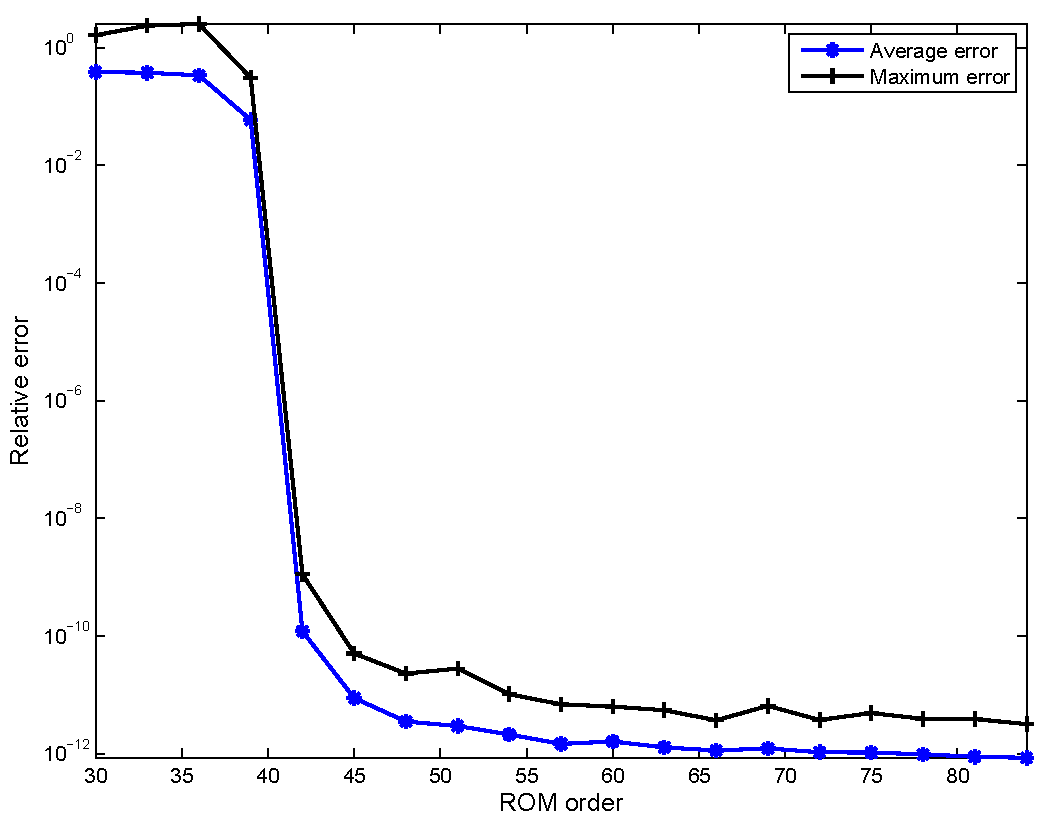
\includegraphics[width=12cm]{vivaldi3dError} 
\caption{Error for several orders of ROM able to scan the whole three-dimensional space.}
\label{fig:vivaldi3dError}
\end{figure}
\begin{figure}[hbpt!]
\centering
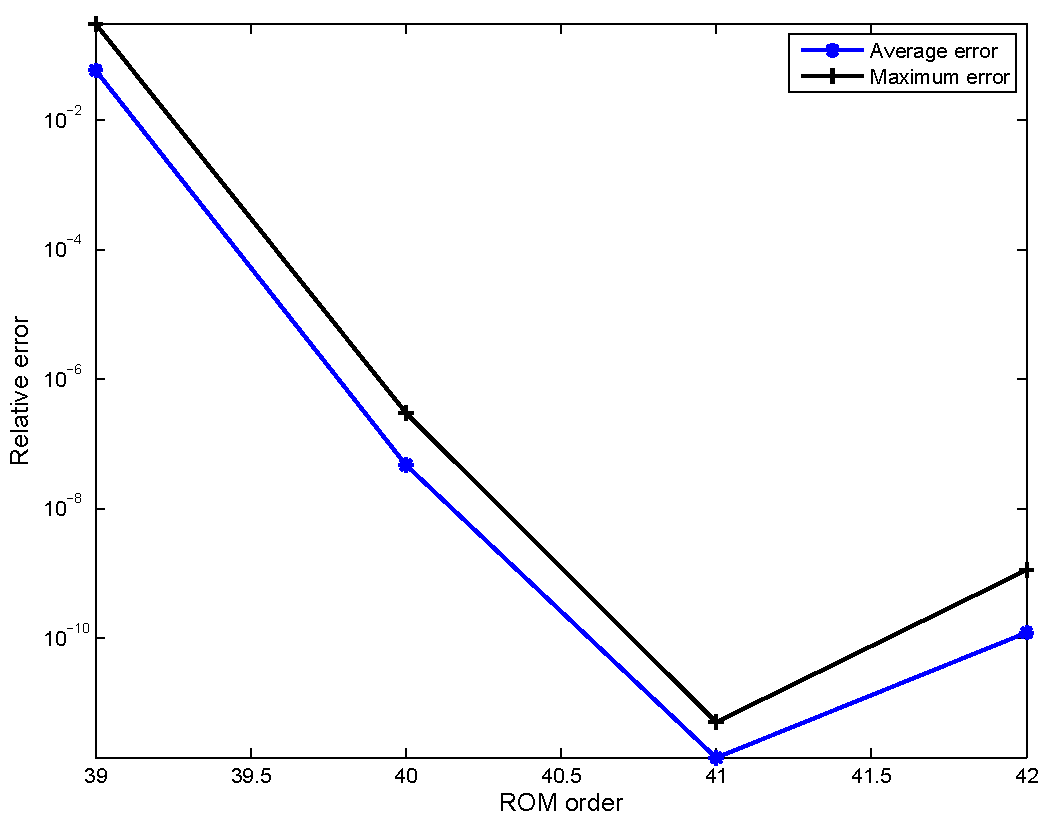
\includegraphics[width=12cm]{vivaldi3dErrorZoom} 
\caption{Error for 39, 40, 41 and 42 ROM orders.}
\label{fig:vivaldi3dErrorZoom}
\end{figure}
